\documentclass[bachelor, och, pract, times]{SCWorks}
% параметр - тип обучения - одно из значений:
%    spec     - специальность
%    bachelor - бакалавриат (по умолчанию)
%    master   - магистратура
% параметр - форма обучения - одно из значений:
%    och   - очное (по умолчанию)
%    zaoch - заочное
% параметр - тип работы - одно из значений:
%    referat    - реферат
%    coursework - курсовая работа (по умолчанию)
%    diploma    - дипломная работа
%    pract      - отчет по практике
%    pract      - отчет о научно-исследовательской работе
%    autoref    - автореферат выпускной работы
%    assignment - задание на выпускную квалификационную работу
%    review     - отзыв руководителя
%    critique   - рецензия на выпускную работу
% параметр - включение шрифта
%    times    - включение шрифта Times New Roman (если установлен)
%               по умолчанию выключен 

\usepackage[T2A]{fontenc}
\usepackage[utf8]{inputenc}
\usepackage{graphicx}
\usepackage[sort,compress]{cite}
\usepackage{amsmath}
\usepackage{amssymb}
\usepackage{amsthm}
\usepackage{fancyvrb}
\usepackage{longtable}
\usepackage{array}
\usepackage{makecell}
\usepackage{multirow}
\usepackage[english,russian]{babel}

\usepackage{tempora}
\usepackage[hidelinks]{hyperref}

\usepackage{pgfplots}
\usepackage{tikz}
\usepackage{float}
\pgfplotsset{compat = newest}

\usepackage{minted}
\setminted[c++]{linenos, breaklines = true, style = bw, fontsize = \small}


\newcommand{\eqdef}{\stackrel {\rm def}{=}}

\newtheorem{lem}{Лемма}

\begin{document}


% Кафедра (в родительном падеже)
\chair{математической кибернетики и компьютерных наук}
% Руководитель ДПП ПП для цифровой кафедры (перекрывает заведующего кафедры)
% \chpretitle{ заведующий кафедрой математических основ информатики и олимпиадного\\ программирования на базе МАОУ <<Ф"=Т лицей №1>>
% }
\chtitle{г. Саратов, к.\,ф.-м.\,н., доцент}
\chname{С.\,В.\,Миронов}

% Научный руководитель (для реферата преподаватель проверяющий работу)
\satitle{доцент, к.\,ф.-м.\,н.} %должность, степень, звание
\saname{М.\,И.\,Сафрончик}
\satitle{доцент, к.\,ф.-м.\,н.} %должность, степень, звание Руководитель практики от организации (руководитель для цифровой кафедры)
\patitle{доцент, к.\,ф.-м.\,н.}
\paname{М.\,И.\,Сафрончик}

% Семестр (только для практики, для остальных типов работ не используется)
\term{3}

% Наименование практики (только для практики, для остальных типов работ не
% используется)
\practtype{учебная (рассредоточенная)}

% Продолжительность практики (количество недель) (только для практики, для
% остальных типов работ не используется)
\duration{18}

% Даты начала и окончания практики (только для практики, для остальных типов
% работ не используется)
\practStart{02.09.24}
\practFinish{12.01.25}
% Тема работы
\title{Разработка приложений Windows.Forms на языке C++ в среде Microsoft Visual Studio}

% Курс
\course{2}

% Группа
\group{251}

% Факультет (в родительном падеже) (по умолчанию "факультета КНиИТ")
%\department{факультета КНиИТ}

% Специальность/направление код - наименование

\napravlenie{09.03.04 "--- Программная инженерия}

% Фамилия, имя, отчество в родительном падеже
\author{Соловьева Артема Сергеевича}

% Год выполнения отчета
\date{2024}

\maketitle

% Включение нумерации рисунков, формул и таблиц по разделам
% (по умолчанию - нумерация сквозная)
% (допускается оба вида нумерации)
%\secNumbering

\tableofcontents
\intro 

Целью практики является освоение механизма построения оконного интерфейса приложений в среде Microsoft Visual Studio на языке C++/CLI с использованием .NET Framework и Windows Forms. В результате прохождения практики должны быть отработаны следующие навыки:
\begin{itemize}
    \item Создание нового проекта;
    \item Добавление и настройка элементов управления;
    \item проверка пользовательского ввода данных для решения поставленной задачи, обработка ошибок ввода;
    \item разработка алгоритма решения поставленной задачи с использованием оконного интерфейса;
    \item тестирование приложения;
    \item документирование разработанного кода.
\end{itemize}
% Оптимизация от Дани

\section{Вычисление факториала}

\subsection{Условие задания}

Разработать приложение для вычисления факториала по приведенному примеру. 

Приложение должно содержать следующие компоненты:
\begin{enumerate}
    \item Заголовок формы должен отражать суть задания.
    \item Все элементы формы должны быть внятно подписаны (кнопки подписаны, у текстового поля должно быть написано, для чего оно нужно и т. д.)
    \item В коде должны быть комментарии и отступы (код должен быть легко читаем).
    \item В коде программы все элементы формы должны быть переименованы (btnName -  для кнопок, lblName - для ссылок, txtName - для текстового поля и т. д.) Наименования должны быть понятными.
    \item Приложение должно корректно работать (выводить ответ или ошибку с соответствующим сообщением) для следующих данных: ввод буквы, ввод отрицательного числа, ввод нуля, ввод положительного числа (< 10), ввод большого положительного числа. После вывода ошибок при вводе корректных данных поля ошибок должны очищаться.  
\end{enumerate}


\subsection{Вид формы в конструкторе}

Создано окно приложения, содержащее два элемента TextBox, два элемента
Label и один элемент Button. Вид окна представлен на рисунке \ref{task1_form} \cite{лаврентьев2020использование}. 

\begin{figure}[H]
    \centering
    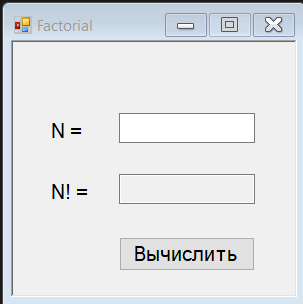
\includegraphics[width=0.3\linewidth]{lections/img/task1_form.png}
    \caption{Окно приложения <<factorial>> открытое в конструкторе }
    \label{task1_form}
\end{figure}


\subsection{Таблица с описанием переименованных элементов формы}
Все измененные элементы формы указаны в таблице \ref{task1_attributes}.
\begin{table}[H]
\caption{Значения атрибутов элементов в приложении factorial}
\begin{tabular}{|l|l|l|}
\hline
\textbf{\begin{tabular}[c]{@{}l@{}}Описание элементов\\ формы\end{tabular}}         & \textbf{\begin{tabular}[c]{@{}l@{}}Список измененных\\ атрибутов\end{tabular}} & \textbf{\begin{tabular}[c]{@{}l@{}}Новое значение\\ атрибута\end{tabular}} \\ \hline
\multirow{3}{*}{Форма MyForm}                                                       & FormBorderStyle                                                                & Fixed3D                                                                    \\ \cline{2-3} 
                                                                                    & Text                                                                           & Factorial                                                                  \\ \cline{2-3} 
                                                                                    & MaximizeBox                                                                    & False                                                                      \\ \hline
TextBox ввод числа                                                                  & Name                                                                           & input                                                                      \\ \hline
\multirow{2}{*}{\begin{tabular}[c]{@{}l@{}}TextBox вывод\\ факториала\end{tabular}} & Name                                                                           & output                                                                     \\ \cline{2-3} 
                                                                                    & ReadOnly                                                                       & True                                                                       \\ \hline
\multirow{2}{*}{Label у поля ввода}                                                 & Name                                                                           & lblin                                                                      \\ \cline{2-3} 
                                                                                    & Text                                                                           & N =                                                                        \\ \hline
\multirow{2}{*}{Label у поля вывода}                                                & Name                                                                           & lblout                                                                     \\ \cline{2-3} 
                                                                                    & Text                                                                           & N! =                                                                       \\ \hline
\multirow{2}{*}{Кнопка "Вычислить"}                                                 & Name                                                                           & solve                                                                      \\ \cline{2-3} 
                                                                                    & Text                                                                           & Вычислить                                                                  \\ \hline
\end{tabular}

\label{task1_attributes}
\end{table}


\subsection{Примеры правильной и неправильной работы}
После запуска программы на экране появляется окно на рисунке \ref{task1_launch1}.
\begin{figure}[H]
    \centering
    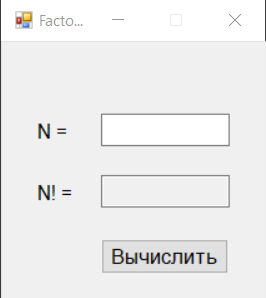
\includegraphics[width=0.4\linewidth]{lections/img/task1_launch1.png}
    \caption{Запуск программы}
    \label{task1_launch1}
\end{figure}
При вводе числа в поле ввода и нажатии на кнопку "Вычислить" (на рисунке \ref{task1_launch2})
\begin{figure}[H]
    \centering
    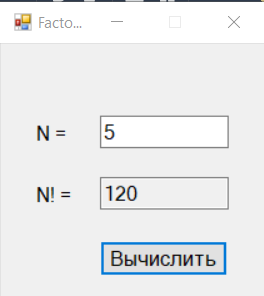
\includegraphics[width=0.4\linewidth]{lections/img/task1_launch2.png}
    \caption{Вычисление факториала}
    \label{task1_launch2}
\end{figure}
При попытке ввода не числа, программа выведет ошибку (на рисунке \ref{task1_launch3})
\begin{figure}[H]
    \centering
    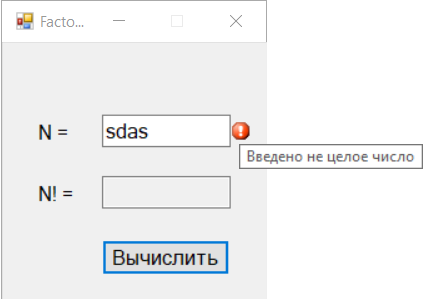
\includegraphics[width=0.4\linewidth]{lections/img/task1_launch3.png}
    \caption{Ошибка формата ввода}
    \label{task1_launch3}
\end{figure}
\subsection{Примеры исходного кода}

Код, выполняющийся при нажатии на кнопку "Вычислить".
\begin{minted}[style=bw,
 linenos=true,
 breaklines=true,
 numbersep=5pt,
 tabsize=2,
 fontsize=\small,
 bgcolor=white]{cpp}
private: System::Void solve_Click(System::Object^ sender, System::EventArgs^ e) {
	this->output->Text = "";
	errorProvider1->SetError(input, String::Empty);
	long long InputNumber;
	bool result = Int64::TryParse(this->input->Text, InputNumber); //переводим строку из TextBox число
	if (!result) { //dвели не число
		errorProvider1->SetError(input, "Введено не целое число");
	}
	else {//число
		if (InputNumber > 20) {
			this->output->Text = "Слишком большое число";
		}
		else {
			long long OutputNumber = fact(InputNumber);//результат
			if (OutputNumber == -1) { //отрицательное число
				errorProvider1->SetError(input, "Введено отрицательное число");
			}
			else { //все нормально
				this->output->Text = System::Convert::ToString(OutputNumber);//записываем в поле вывода
			}
		}
	}
}
\end{minted}
Другие фрагменты кода расположены в приложении \ref{app:factorial}.
\sectionbreak
\section{Простые вычисления}

\subsection{Условие задания}
Выполнить задание. Номер варианта задает преподавателем. 

Проверить работу созданного приложения на приведенных тестовых примерах. Тесты сделаны на Visual Studio 2008, поэтому обращайте внимание только на первые шесть цифр после запятой.

Приложение должно содержать следующие компоненты:
\begin{enumerate}
    \item Заголовок формы должен отражать суть задания.
    \item Все элементы формы должны быть внятно подписаны (кнопки подписаны, у текстового поля должно быть написано, для чего оно нужно и т. д.)
    \item В коде должны быть комментарии и отступы (код должен быть легко читаем).
    \item Должна быть проверка ошибок - ввод не числа, ввод числа, находящегося за пределами ОДЗ, ввод числа, принадлежащего ОДЗ.
    \item Если надо ввести 2 значения, то в случае ввод букв в оба поля, ошибка должна быть у обоих полей; в случае ввода одной буквы - только у того поля, где буква.
\end{enumerate}

\textbf{Вариант 4.} Смотреть на рисунке \ref{task2_var4}.
\begin{figure}[H]
    \centering
    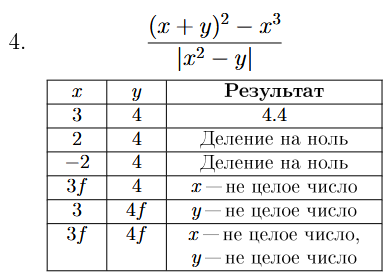
\includegraphics[width=0.5\linewidth]{lections/img/task2_var4.png}
    \caption{Задание 2 Вариант 4}
    \label{task2_var4}
\end{figure}

\subsection{Вид формы в конструкторе}
Создано окно приложения, содержащее три элемента TextBox, три элемента
Label, один элемент Button и один элемент ErrorProvider для обработки ошибок. Вид окна представлен на рисунке \ref{task2_form} \cite{никлаус2022алгоритмы}.
\begin{figure}[H]
    \centering
    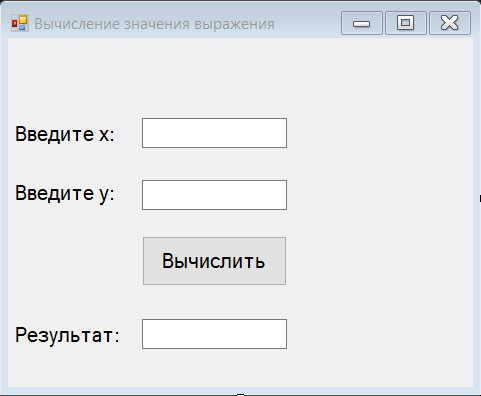
\includegraphics[width=0.5\linewidth]{lections/img/task2_form.png}
    \caption{Окно приложения «Вычисление значения выражения» открытое в конструкторе}
    \label{task2_form}
\end{figure}


\subsection{Таблица с описанием переименованных элементов формы}
Все измененные элементы формы указаны в таблице \ref{task2_attributes}.

\begin{table}[H]
\caption{Значения атрибутов элементов в приложении <<Вычисление значения выражения>>}
\begin{tabular}{|l|l|l|}
\hline
\textbf{\begin{tabular}[c]{@{}l@{}}Описание элементов\\ формы\end{tabular}} & \textbf{\begin{tabular}[c]{@{}l@{}}Список измененных\\ атрибутов\end{tabular}} & \textbf{\begin{tabular}[c]{@{}l@{}}Новое значение\\ атрибута\end{tabular}} \\ \hline
Форма MyForm                                                                & Text                                                                           & \begin{tabular}[c]{@{}l@{}}Вычисление значений\\ выражения\end{tabular}    \\ \hline
TextBox ввода x                                                             & Name                                                                           & x\_input                                                                   \\ \hline
TextBox ввода y                                                             & Name                                                                           & y\_input                                                                   \\ \hline
\begin{tabular}[c]{@{}l@{}}TextBox вывод\\ результата\end{tabular}          & Name                                                                           & output                                                                     \\ \hline
\multirow{2}{*}{Label у поля ввода x}                                       & Name                                                                           & x\_lbl                                                                     \\ \cline{2-3} 
                                                                            & Text                                                                           & Введите x:                                                                 \\ \hline
\multirow{2}{*}{Label у поля ввода y}                                       & Name                                                                           & y\_lbl                                                                     \\ \cline{2-3} 
                                                                            & Text                                                                           & Введите y:                                                                 \\ \hline
\multirow{2}{*}{Label у поля вывода}                                        & Name                                                                           & res\_lbl                                                                   \\ \cline{2-3} 
                                                                            & Text                                                                           & Результат                                                                  \\ \hline
\multirow{2}{*}{Кнопка "Вычислить"}                                         & Name                                                                           & solvebtn                                                                   \\ \cline{2-3} 
                                                                            & Text                                                                           & Вычислить                                                                  \\ \hline
\end{tabular}

\label{task2_attributes}
\end{table}


\subsection{Примеры правильной и неправильной работы}
После запуска программы на экране появляется окно на рисунке \ref{task2_launch1}.
\begin{figure}[H]
    \centering
    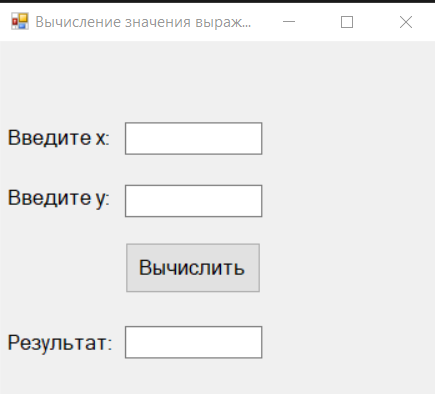
\includegraphics[width=0.4\linewidth]{lections/img/task2_launch1.png}
    \caption{Запуск программы}
    \label{task2_launch1}
\end{figure}
При вводе x и y в соответствующие поля и нажатии на кнопку "Вычислить" (на рисунке \ref{task2_launch2})
\begin{figure}[H]
    \centering
    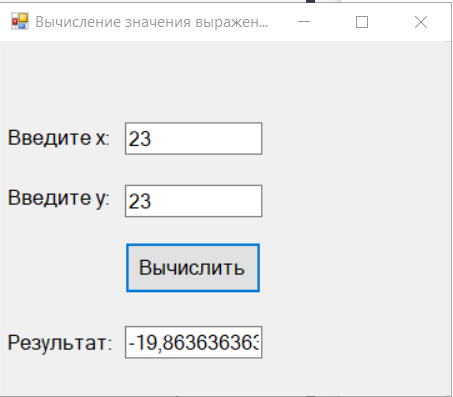
\includegraphics[width=0.4\linewidth]{lections/img/task2_launch2.png}
    \caption{Вычисление выражения}
    \label{task2_launch2}
\end{figure}
При попытке вычисления выражения такого, что $x^2 - y = 0$, вылезает ошибка <<деление на ноль>>  в поле вывода. (на рисунке \ref{task2_launch3}).
\begin{figure}[H]
    \centering
    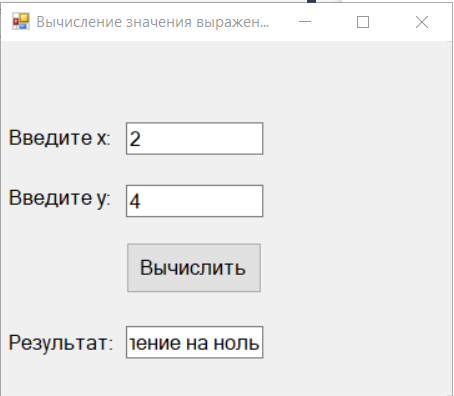
\includegraphics[width=0.4\linewidth]{lections/img/task2_launch3.png}
    \caption{Ошибка деления на ноль}
    \label{task2_launch3}
\end{figure}

\subsection{Примеры исходного кода}
Начало функции, выполняющейся при нажатии на кнопку <<Вычислить>>.
\begin{minted}[style=bw,
 linenos=true,
 breaklines=true,
 numbersep=5pt,
 tabsize=2,
 fontsize=\small,
 bgcolor=white]{cpp}
private: System::Void solvebtn_Click(System::Object^ sender, System::EventArgs^ e) {
	this->output->Text = ""; // Стираем поле вывода

	errors->SetError(x_input, String::Empty); // обнуляем ошибки
	errors->SetError(y_input, String::Empty);

	Int64 x, y; // Переменные для считывания полей ввода
	double result; // переменная для записи результата

	bool result_x = Int64::TryParse(this->x_input->Text, x); // записываем из полей ввода в соответствующие переменные
	bool result_y = Int64::TryParse(this->y_input->Text, y); // и проверяем на успешность выполнения парсинга

	if (!result_x) { // если неудачно
		errors->SetError(x_input, "Введено не целое число");
	}
	if (!result_y) {
		errors->SetError(y_input, "Введено не целое число");
	}
	if (result_x && result_y) { // если удачно
		if (x * x - y == 0) { // проверка на ОДЗ
			this->output->Text = "Деление на ноль";
		}
		else {
			result = (1.0) * ((x + y) * (x + y) - x * x * x) / (std::abs(x * x - y)); //Считаем
			this->output->Text = System::Convert::ToString(result); //Записываем результат
		}
	}
}
\end{minted}
Другие фрагменты кода расположены в приложении \ref{app:simple_calculations}.
\sectionbreak
\section{Рекурсивные вычисления}

\subsection{Условие задания}

Разработать приложение для выполнения своего варианта задания. Номер варианта задается преподавателем.

Проверить работу приложения на приведенных тестах.

Приложение должно содержать следующие компоненты:

\begin{enumerate}
    \item Заголовок формы должен отражать суть задания.
    \item Все элементы формы должны быть внятно подписаны (кнопки подписаны, у текстового поля должно быть написано, для чего оно нужно и т. д.)
    \item В коде должны быть комментарии и отступы (код должен быть легко читаем).
    \item В коде программы все элементы формы должны быть переименованы (btnName -  для кнопок, lblName - для ссылок, txtName - для текстового поля и т. д.) Наименования должны быть понятными.
    \item Приложение должно корректно работать (выводить ответ или ошибку с соответствующим сообщением) для следующих данных: ввод буквы, ввод отрицательного числа, ввод нуля, ввод положительного числа (< 10), ввод большого положительного числа. После вывода ошибок при вводе корректных данных поля ошибок должны очищаться.
\end{enumerate}

\textbf{Вариант 5.} Смотреть на рисунке \ref{task3_var5}.
\begin{figure}[H]
    \centering
    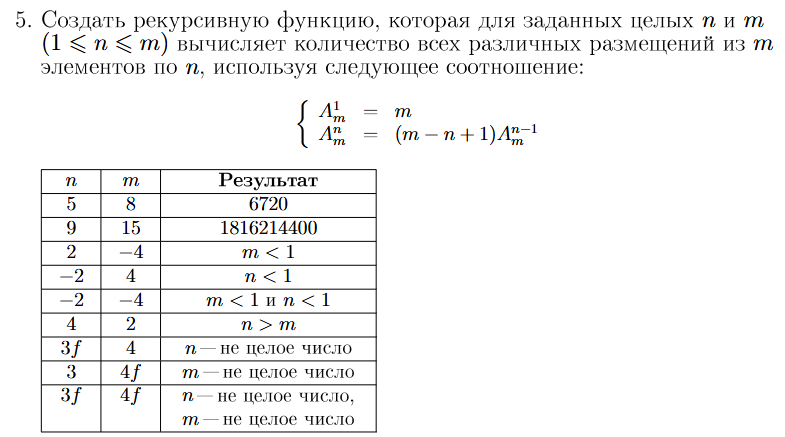
\includegraphics[width=0.9\linewidth]{lections/img/task3_var5.png}
    \caption{Задание 3 Вариант 5}
    \label{task3_var5}
\end{figure}

\subsection{Вид формы в конструкторе}

Создано окно приложения, содержащее три элемента TextBox, два элемента
Label, один элемент Button. Один из элментов TextBox содержит атрибут Multiline. Вид окна представлен на рисунке \ref{task3_form} \cite{комракова2022приложение}.
\begin{figure}[H]
    \centering
    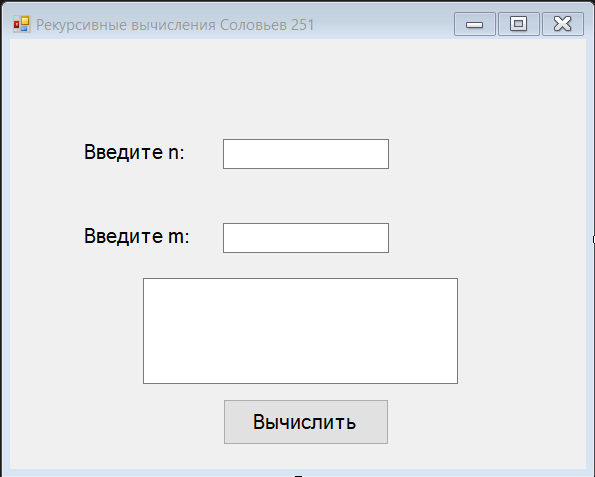
\includegraphics[width=0.8\linewidth]{lections/img/task3_form.png}
    \caption{Окно приложения «Рекурсивные вычисления» открытое в конструкторе}
    \label{task3_form}
\end{figure}

\subsection{Таблица с описанием переименованных элементов формы}
Все измененные элементы формы указаны в таблице \ref{task3_attributes}.


\begin{table}[H]
\caption{Значения атрибутов элементов в приложении <<Рекурсивные вычисления>>}
\begin{tabular}{|l|l|l|}
\hline
\textbf{\begin{tabular}[c]{@{}l@{}}Описание элементов\\ формы\end{tabular}} & \textbf{\begin{tabular}[c]{@{}l@{}}Список измененных\\ атрибутов\end{tabular}} & \textbf{\begin{tabular}[c]{@{}l@{}}Новое значение\\ атрибута\end{tabular}}    \\ \hline
Форма MyForm                                                                & Text                                                                           & \begin{tabular}[c]{@{}l@{}}Рекурсивные вычисления\\ Соловьев 251\end{tabular} \\ \hline
TextBox ввода n                                                             & Name                                                                           & n\_input                                                                      \\ \hline
TextBox ввода m                                                             & Name                                                                           & m\_input                                                                      \\ \hline
\multirow{2}{*}{TextBox вывода}                                             & Name                                                                           & Output                                                                        \\ \cline{2-3} 
                                                                            & Multiline                                                                      & True                                                                          \\ \hline
\multirow{2}{*}{Label у поля ввода n}                                       & Name                                                                           & n\_inputlbl                                                                   \\ \cline{2-3} 
                                                                            & Text                                                                           & Введите n:                                                                    \\ \hline
\multirow{2}{*}{Label у поля ввода m}                                       & Name                                                                           & m\_inputlbl                                                                   \\ \cline{2-3} 
                                                                            & Text                                                                           & Введите m:                                                                    \\ \hline
\multirow{2}{*}{Кнопка "Вычислить"}                                         & Name                                                                           & Solve                                                                         \\ \cline{2-3} 
                                                                            & Text                                                                           & Вычислить                                                                     \\ \hline
\end{tabular}

\label{task3_attributes}
\end{table}


\subsection{Примеры правильной и неправильной работы}
После запуска программы на экране появляется окно на рисунке \ref{task3_launch1}.
\begin{figure}[H]
    \centering
    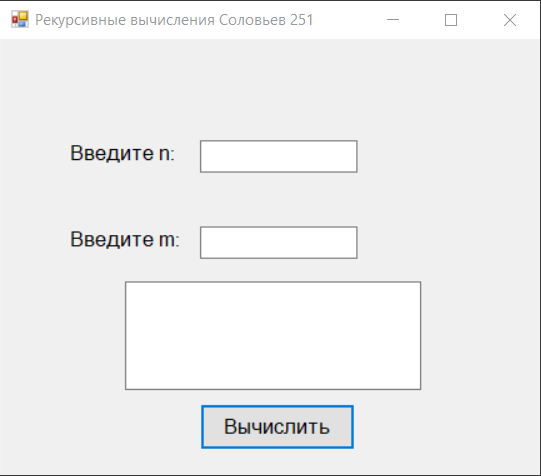
\includegraphics[width=0.6\linewidth]{lections/img/task3_launch1.png}
    \caption{Запуск программы}
    \label{task3_launch1}
\end{figure}

При вводе удовлетворяющих условиям n и m в соответствующие поля и нажатии на кнопку <<Вычислить>> (на рисунке \ref{task3_launch2}).
\begin{figure}[H]
    \centering
    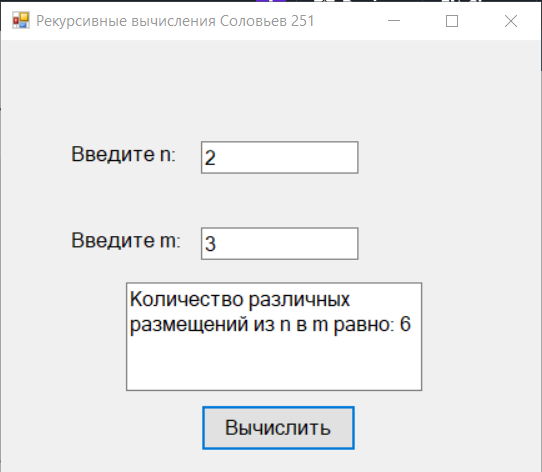
\includegraphics[width=0.6\linewidth]{lections/img/task3_launch2.png}
    \caption{Вычисление выражения}
    \label{task3_launch2}
\end{figure}

При попытке ввода не числа, программа выведет ошибку (на рисунке \ref{task3_launch3})
\begin{figure}[H]
    \centering
    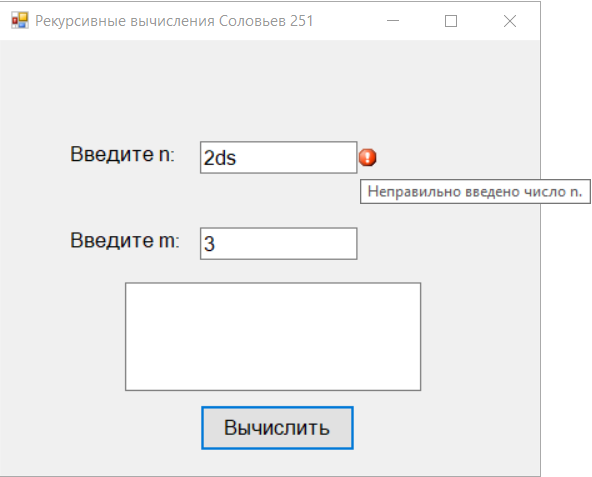
\includegraphics[width=0.7\linewidth]{lections/img/task3_launch3.png}
    \caption{Ошибка формата ввода}
    \label{task3_launch3}
\end{figure}

\subsection{Примеры исходного кода}

Функция вычисления числа перестановок.
\begin{minted}[style=bw,
 linenos=true,
 breaklines=true,
 numbersep=5pt,
 tabsize=2,
 fontsize=\small,
 bgcolor=white]{cpp}
long long per(long long n, long long m) {
	if (n == 1) return m;
	else return (m - n + 1) * per(n - 1, m);
}
\end{minted}
Другие фрагменты кода расположены в приложении \ref{app:recursive_calculations}.
\sectionbreak
\section{Обработка табличных данных. Часть 1 }

\subsection{Условие задания}
Создать приложение для выполнения задания. Использовать элемент формы DataGridView. 

\textbf{ДИАПАЗОН [a,b] означает, что mas[i][j] >= a \&\& mas[i][j] <= b.}

Приложение должно выполнять следующие действия:

\begin{enumerate}
    \item Возможность удалять и добавлять строки таблицы. Проект не должен аварийно завершаться при удалении несуществующей таблицы.
    \item Проверять ввод не числовых данных как в таблицу, так и в остальные текстовые поля (если есть в задании).
    \item Если есть диапазон значений [a,b], проверять, что a < b.
    \item Заголовок формы должен отражать суть задания.
    \item Все элементы формы должны быть внятно подписаны (кнопки подписаны, у тестового поля должно быть написано, для чего оно нужно и т. д.)
    \item В коде должны быть комментарии и отступы (код должен быть легко читаем).
    \item В коде программы все элементы формы должны быть переименованы (btnName -  для кнопок, lblName - для ссылок, txtName - для текстового поля и т. д.) Наименования должны быть понятными.
    \item Приложение должно корректно работать (выводить ответ или ошибку с соответствующим сообщением). После вывода ошибок при вводе корректных данных поля ошибок должны очищаться.  
\end{enumerate}

\textbf{Вариант 9.} Смотреть на рисунке \ref{task4_var9}.
\begin{figure}[H]
    \centering
    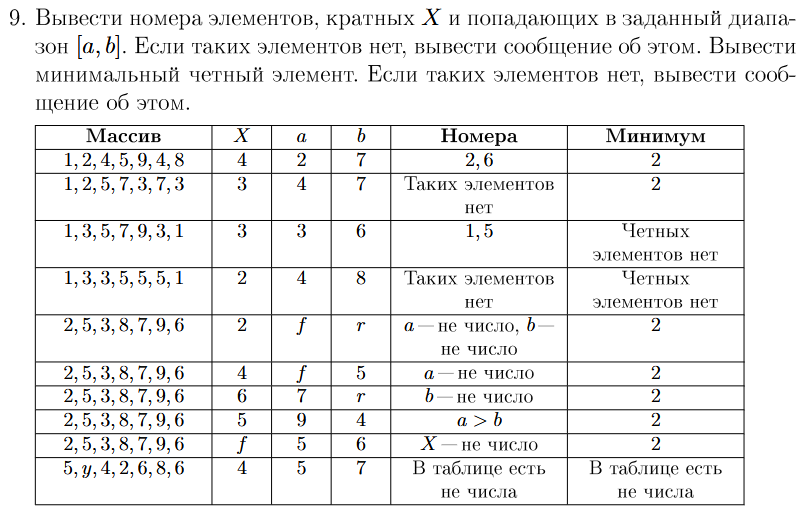
\includegraphics[width=0.9\linewidth]{lections/img/task4_var9.png}
    \caption{Задание 4 Вариант 9}
    \label{task4_var9}
\end{figure}

\subsection{Вид формы в конструкторе}

Создано окно приложения, содержащее пять элементов TextBox, четыре элемента Label, четыре элемента Button, один элемент gridview и один элемент ErrorProvider для обработки ошибок. Вид окна представлен на рисунке \ref{task4_form} \cite{ахо2000структуры}.
\begin{figure}[H]
    \centering
    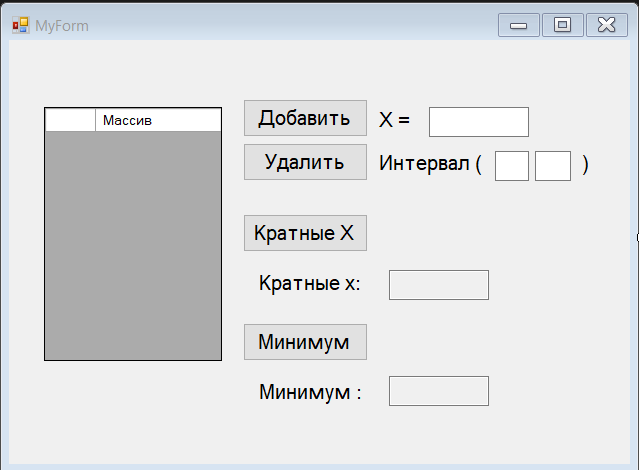
\includegraphics[width=0.8\linewidth]{lections/img/task4_form.png}
    \caption{Окно приложения «Обработка табличных данных. Часть 1» открытое в конструкторе}
    \label{task4_form}
\end{figure}


\subsection{Таблица с описанием переименованных элементов формы}
Все измененные элементы формы указаны в таблице \ref{task4_attributes}.


\begin{table}[H]
\caption{Значения атрибутов элементов в приложении <<Обработка табличных данных. Часть 1>>}
\begin{tabular}{|l|l|l|}
\hline
\textbf{\begin{tabular}[c]{@{}l@{}}Описание элементов\\ формы\end{tabular}} & \textbf{\begin{tabular}[c]{@{}l@{}}Список измененных\\ атрибутов\end{tabular}} & \textbf{\begin{tabular}[c]{@{}l@{}}Новое значение\\ атрибута\end{tabular}}    \\ \hline
Форма MyForm                                                                & Text                                                                           & \begin{tabular}[c]{@{}l@{}}Обработка табличных\\ данных. Часть 1\end{tabular} \\ \hline
TextBox ввода X                                                             & Name                                                                           & x\_input                                                                      \\ \hline
TextBox ввода начала интервала                                              & Name                                                                           & int\_a                                                                        \\ \hline
TextBox ввода конца интервала                                               & Name                                                                           & int\_b                                                                        \\ \hline
\multirow{2}{*}{TextBox вывода кратных х}                                   & Name                                                                           & krat\_box                                                                     \\ \cline{2-3} 
                                                                            & ReadOnly                                                                       & True                                                                          \\ \hline
\multirow{2}{*}{TextBox вывода минимума}                                    & Name                                                                           & chet\_box                                                                     \\ \cline{2-3} 
                                                                            & ReadOnly                                                                       & True                                                                          \\ \hline
Кнопка "Добавить"                                                           & Name                                                                           & mas\_add                                                                      \\ \hline
                                                                            & Text                                                                           & Добавить                                                                      \\ \hline
\multirow{2}{*}{Кнопка "Удалить"}                                           & Name                                                                           & mas\_pop                                                                      \\ \cline{2-3} 
                                                                            & Text                                                                           & Удалить                                                                       \\ \hline
\multirow{2}{*}{Кнопка "Кратные X"}                                         & Name                                                                           & krat\_btn                                                                     \\ \cline{2-3} 
                                                                            & Text                                                                           & Кратные Х                                                                     \\ \hline
\multirow{2}{*}{Кнопка "Минимум"}                                           & Name                                                                           & min\_btn                                                                      \\ \cline{2-3} 
                                                                            & Text                                                                           & Минимум                                                                       \\ \hline
\multirow{3}{*}{Таблица ввода}                                              & Name                                                                           & mas\_grid                                                                     \\ \cline{2-3} 
                                                                            & AllowUserToAddRows                                                             & False                                                                         \\ \cline{2-3} 
                                                                            & AllowUserToDeleteRows                                                          & False                                                                         \\ \hline
\end{tabular}
\label{task4_attributes}
\end{table}

\subsection{Примеры правильной и неправильной работы}
После запуска программы на экране появляется окно на рисунке \ref{task4_launch1}.
\begin{figure}[H]
    \centering
    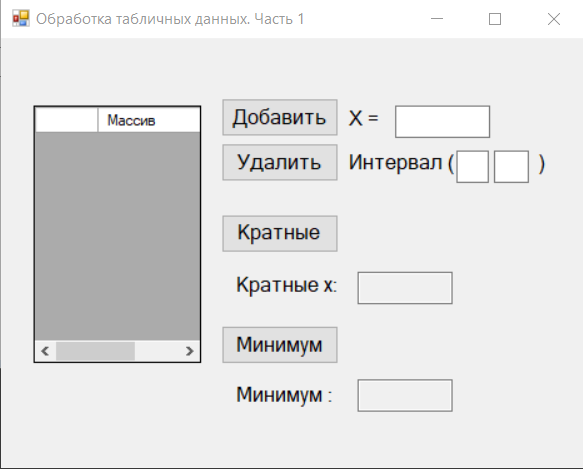
\includegraphics[width=0.6\linewidth]{lections/img/task4_launch1.png}
    \caption{Запуск программы}
    \label{task4_launch1}
\end{figure}


При вводе целого X в поле ввода и нажатии на кнопку <<Добавить>> (на рисунке \ref{task4_launch2}).
\begin{figure}[H]
    \centering
    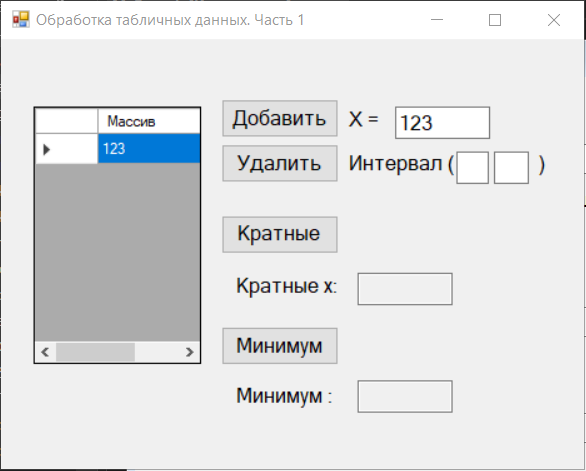
\includegraphics[width=0.6\linewidth]{lections/img/task4_launch2.png}
    \caption{Вычисление выражения}
    \label{task4_launch2}
\end{figure}

При попытке ввода не числа, программа выведет ошибку (на рисунке \ref{task4_launch3})
\begin{figure}[H]
    \centering
    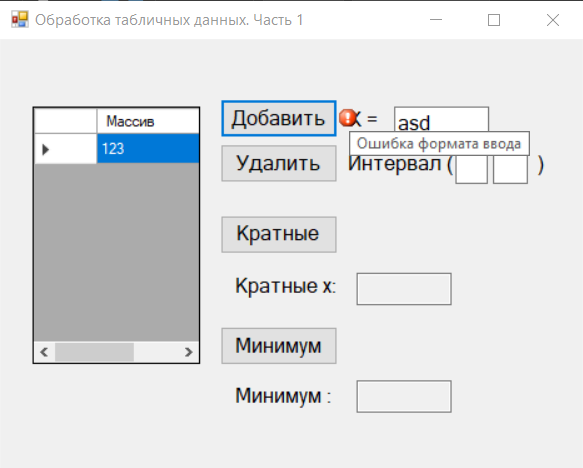
\includegraphics[width=0.7\linewidth]{lections/img/task4_launch3.png}
    \caption{Ошибка формата ввода}
    \label{task4_launch3}
\end{figure}

\subsection{Примеры исходного кода}


Функция при нажатии на кнопку "Кратные Х".
\begin{minted}[style=bw,
 linenos=true,
 breaklines=true,
 numbersep=5pt,
 tabsize=2,
 fontsize=\small,
 bgcolor=white]{cpp}
private: System::Void krat_btn_Click(System::Object^ sender, System::EventArgs^ e) {
	this->errorProvider1->Clear();
	this->krat_box->Text = "";
	long long x,y,a,b;
	bool result = Int64::TryParse(this->x_input->Text, x);
	bool resulta = Int64::TryParse(this->int_a->Text, a);
	bool resultb = Int64::TryParse(this->int_b->Text, b);
	if (!result) {
		this->errorProvider1->SetError(this->x_input, "Неправильный формат числа X");
		return;
	}
	if (!resulta || !resultb) {
		this->errorProvider1->SetError(this->int_a, "Неправильный формат границ интервала");
		return;
	}
	bool found_krat = false;
	for (int i = a; i < this->mas_grid->RowCount && i < b; i++) {
		result = Int64::TryParse(this->mas_grid->Rows[i]->Cells[0]->Value->ToString(), y);
		if (y % x == 0) {
			found_krat = true;
			this->krat_box->Text += System::Convert::ToString(i+1) + ", ";
		}
	}
	if (!found_krat) {
		this->krat_box->Text = "Таких элементов нет";
	}
}
\end{minted}
Другие фрагменты кода расположены в приложении \ref{app:table_data}.
\sectionbreak
\section{Обработка табличных данных. Часть 2 }

\subsection{Условие задания}
Разработать приложение в соответствии со своим вариантом. Номер задания выбирается преподавателем.

Проверить работу приложения на приведенных тестовых примерах.

\textbf{ЗАДАНИЕ ПРЕДПОЛАГАЕТ НАЛИЧИЕ ДВУХ ТАБЛИЦ.} В  первую вводятся данные (должна быть проверка, что введены цифры). Вторую лучше сделать доступной только для чтения. В нее записывается результат. 

\textbf{ФРАЗА "ЗАМЕНИТЬ СТРОКОЙ X"  предполагает, что создается либо таблица, состоящая из одной строки и туда вводятся данные, либо создается текстовое поле, куда вводится число, и вся строка таблицы заменяется этим числом.}

\textbf{ДИАПАЗОН [a,b] означает, что mas[i][j] >= a \&\& mas[i][j] <= b.}

Приложение должно содержать следующие компоненты:
\begin{enumerate}
    \item Заголовок формы должен отражать суть задания.
    \item Все элементы формы должны быть внятно подписаны (кнопки подписаны, у текстового поля должно быть написано, для чего оно нужно и т. д.)
    \item В коде должны быть комментарии и отступы (код должен быть легко читаем).
    \item  Таблица может быть задана двумя способами: 
    \begin{itemize}
        \item либо ввести количество строк и столбцов (тогда необходима проверка, что введено не число) и создать нужную таблицу. При изменении количества строк и столбцов, старая таблица должна быть удалена.
        \item либо добавлять и удалять строки и столбцы с помощью отдельных кнопок. Проследить, чтобы приложение не завершалось аварийно (не удалять нулевую строку).
    \end{itemize}
    \item  Должна быть проверка ошибок - ввод не числа, ввод числа, приводящего к переполнению стека или выхода результата за границы диапазона типа. В таблице также должны быть введены целые числа. В случае ошибочного ввода поля результатов должны автоматически очищаться.
    \item Если данные введены корректно, но отсутствуют необходимые данные (например, надо найти сумму нечетных чисел, а в таблице только четные), то в поле результата должно быть выведено об этом сообщение.
    \item В случае задач с вводом диапазона [a,b] необходима обязательная проверка, что a < b.
\end{enumerate}

\textbf{Вариант 12.} Смотреть на рисунке \ref{task5_var12}.
\begin{figure}[H]
    \centering
    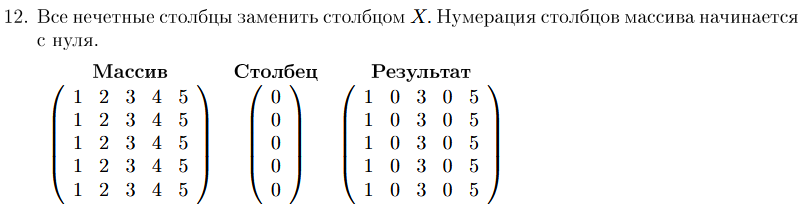
\includegraphics[width=0.9\linewidth]{lections/img/task5_var12.png}
    \caption{Задание 5 Вариант 12}
    \label{task5_var12}
\end{figure}

\subsection{Вид формы в конструкторе}


Создано окно приложения, содержащее два элемента TextBox, три элемента Label, шесть элементов Button, три элемента gridview (один из которых содержит атрибут ReadOnly) и один элемент ErrorProvider для обработки ошибок. Вид окна представлен на рисунке \ref{task5_form} \cite{лафоре2011объектно}.
\begin{figure}[H]
    \centering
    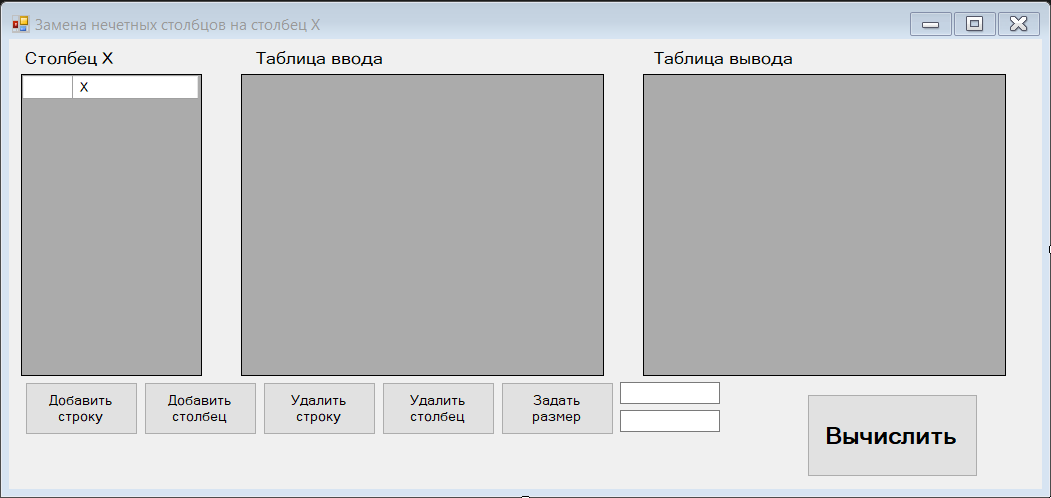
\includegraphics[width=1\linewidth]{lections/img/task5_form.png}
    \caption{Окно приложения «Обработка табличных данных. Часть 2» открытое в конструкторе}
    \label{task5_form}
\end{figure}


\subsection{Таблица с описанием переименованных элементов формы}
Все измененные элементы формы указаны в таблице \ref{task5_attributes}.

\begin{table}[H]
\caption{Значения атрибутов элементов в приложении <<Обработка табличных данных. Часть 2>>}
\begin{tabular}{|l|l|l|}
\hline
\textbf{\begin{tabular}[c]{@{}l@{}}Описание элементов\\ формы\end{tabular}}      & \textbf{\begin{tabular}[c]{@{}l@{}}Список измененных\\ атрибутов\end{tabular}} & \textbf{\begin{tabular}[c]{@{}l@{}}Новое значение\\ атрибута\end{tabular}}    \\ \hline
Форма MyForm                                                                     & Text                                                                           & \begin{tabular}[c]{@{}l@{}}Обработка табличных\\ данных. Часть 2\end{tabular} \\ \hline
\begin{tabular}[c]{@{}l@{}}TextBox ввода количества\\ строк таблицы\end{tabular} & Name                                                                           & set\_size\_lines                                                              \\ \hline
\begin{tabular}[c]{@{}l@{}}TextBox ввода количества\\ Столбцов таблицы\end{tabular} & Name                                                                           & set\_size\_columns                                                            \\ \hline
TextBox ввода конца интервала                                                    & Name                                                                           & int\_b                                                                        \\ \hline
\multirow{2}{*}{TextBox вывода кратных х}                                        & Name                                                                           & krat\_box                                                                     \\ \cline{2-3} 
                                                                                 & ReadOnly                                                                       & True                                                                          \\ \hline
\multirow{2}{*}{TextBox вывода минимума}                                         & Name                                                                           & chet\_box                                                                     \\ \cline{2-3} 
                                                                                 & ReadOnly                                                                       & True                                                                          \\ \hline
\multirow{2}{*}{Кнопка "Добавить строку"}                                        & Name                                                                           & Add\_line                                                                     \\ \cline{2-3} 
                                                                                 & Text                                                                           & Добавить строку                                                               \\ \hline
\multirow{2}{*}{Кнопка "Добавить столбец"}                                       & Name                                                                           & add\_column                                                                   \\ \cline{2-3} 
                                                                                 & Text                                                                           & Добавить столбец                                                              \\ \hline
\multirow{2}{*}{Кнопка "Удалить строку"}                                         & Name                                                                           & remove\_line                                                                  \\ \cline{2-3} 
                                                                                 & Text                                                                           & Удалить строку                                                                \\ \hline
\multirow{2}{*}{Кнопка "Удалить столбец"}                                        & Name                                                                           & remove\_column                                                                \\ \cline{2-3} 
                                                                                 & Text                                                                           & Удалить столбец                                                               \\ \hline
\multirow{2}{*}{Кнопка "Задать размер"}                                          & Name                                                                           & set\_size                                                                     \\ \cline{2-3} 
                                                                                 & Text                                                                           & Задать размер                                                                 \\ \hline
\multirow{2}{*}{Кнопка "Вычислить"}                                              & Name                                                                           & solve\_btn                                                                    \\ \cline{2-3} 
                                                                                 & Text                                                                           & Вычислить                                                                     \\ \hline
\multirow{3}{*}{Таблица ввода столбца X}                                         & Name                                                                           & X\_input                                                                      \\ \cline{2-3} 
                                                                                 & AllowUserToAddRows                                                             & False                                                                         \\ \cline{2-3} 
                                                                                 & AllowUserToDeleteRows                                                          & False                                                                         \\ \hline
\multirow{3}{*}{Таблица ввода матрицы}                                           & Name                                                                           & input\_grid                                                                   \\ \cline{2-3} 
                                                                                 & AllowUserToAddRows                                                             & False                                                                         \\ \cline{2-3} 
                                                                                 & AllowUserToDeleteRows                                                          & False                                                                         \\ \hline
\multirow{4}{*}{Таблица вывода}                                                  & Name                                                                           & output\_grid                                                                  \\ \cline{2-3} 
                                                                                 & AllowUserToAddRows                                                             & False                                                                         \\ \cline{2-3} 
                                                                                 & AllowUserToDeleteRows                                                          & False                                                                         \\ \cline{2-3} 
                                                                                 & ReadOnly                                                                       & True                                                                          \\ \hline
\end{tabular}
\label{task5_attributes}
\end{table}


\subsection{Примеры правильной и неправильной работы}
После запуска программы на экране появляется окно на рисунке \ref{task5_launch1}.
\begin{figure}[H]
    \centering
    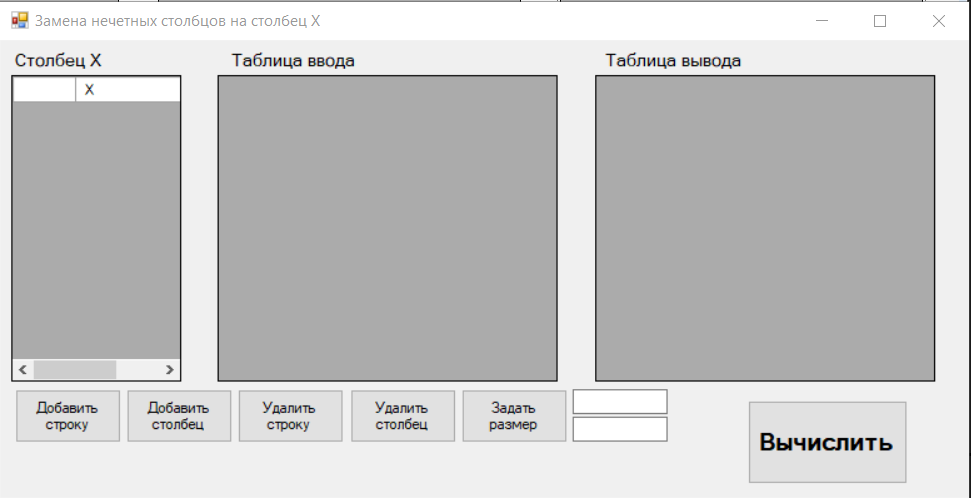
\includegraphics[width=1\linewidth]{lections/img/task5_launch1.png}
    \caption{Запуск программы}
    \label{task5_launch1}
\end{figure}

После ввода столбца X и таблицы ввода и нажатии на кнопку "Вычислить" (на рисунке \ref{task5_launch2}).

\begin{figure}[H]
    \centering
    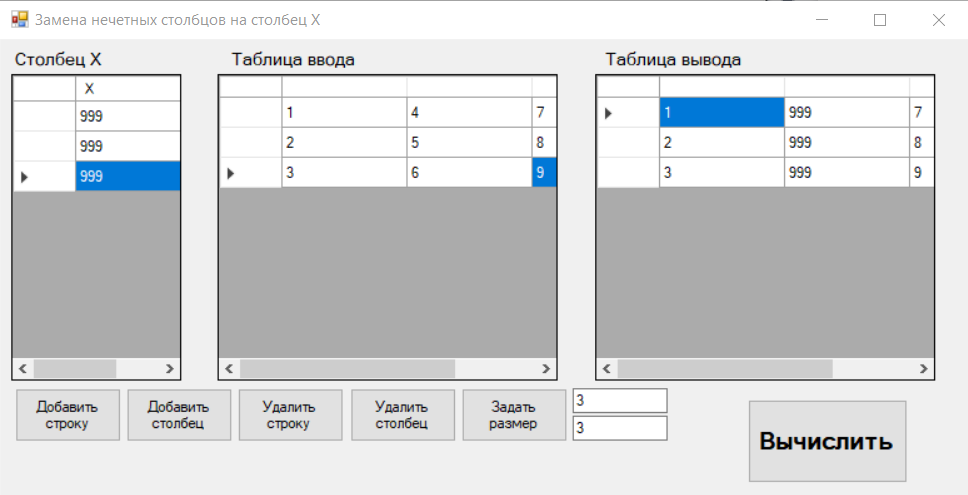
\includegraphics[width=1\linewidth]{lections/img/task5_launch2.png}
    \caption{Замена всех нечетных столбцов столбцом Х (счет начиется с 0)}
    \label{task5_launch2}
\end{figure}

При попытке ввода не числа в таблицу, программа выведет ошибку (на рисунке \ref{task5_launch3})
\begin{figure}[H]
    \centering
    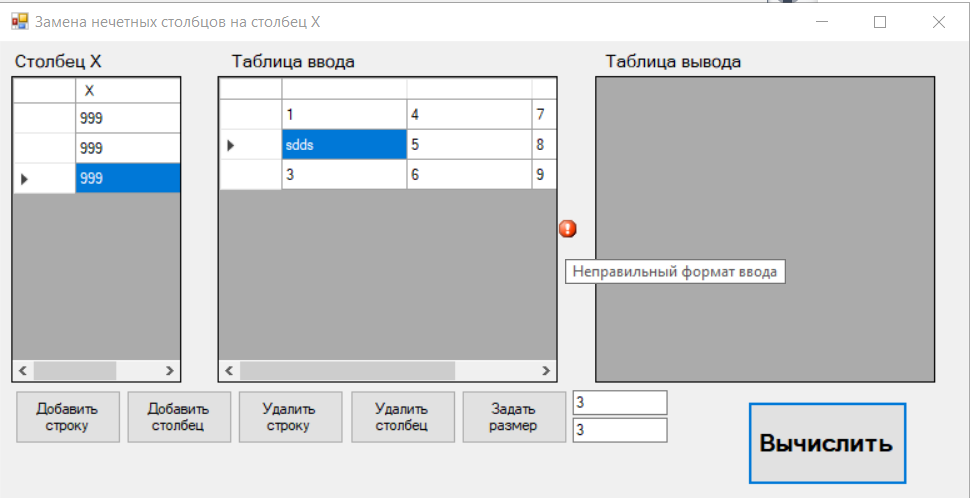
\includegraphics[width=1\linewidth]{lections/img/task5_launch3.png}
    \caption{Ошибка формата ввода}
    \label{task5_launch3}
\end{figure}



\subsection{Примеры исходного кода}


Функция при нажатии на кнопку "Удалить столбец".
\begin{minted}[style=bw,
 linenos=true,
 breaklines=true,
 numbersep=5pt,
 tabsize=2,
 fontsize=\small,
 bgcolor=white]{cpp}
private: System::Void remove_column_Click(System::Object^ sender, System::EventArgs^ e) {
	this->errorProvider1->Clear();
	if (this->input_grid->ColumnCount <= 1 || this->input_grid->RowCount == 0) {
		this->errorProvider1->SetError(remove_column, "Нельзя убрать столбец, которого нет");
		return;
	}
	int i = this->input_grid->CurrentCell->ColumnIndex;
	this->input_grid->Columns->Remove(this->input_grid->Columns[i]);
}
\end{minted}
Другие фрагменты кода расположены в приложении \ref{app:table_data_2}.

\sectionbreak
\section{Матричный калькулятор}

\subsection{Условие задания}

Создать приложение, реализующее основные операции с векторами и матрицами:
\begin{enumerate}
    \item Ввод матрицы, вектора
    \item Создание матриц (единичная, матрица как набор векторов)
    \item Умножение на число, вектор, матрицу
    \item Сложение/вычитание двух матриц
    \item Сложение/вычитание двух векторов
    \item Скалярное и векторное произведение двух векторов
    \item Транспонированная матрица
    \item Определитель, ранг матрицы
\end{enumerate}
Выводить сообщения об ошибках (ввод не числа, несоответствие размерностей)

\subsection{Вид формы в конструкторе}



Создано окно приложения, содержащее пять элементов TextBox, четыре элемента Label, четыре элемента Button, один элемент gridview и один элемент ErrorProvider для обработки ошибок. Вид окна представлен на рисунке \ref{task6_form} \cite{stroustrup2013c++}.
\begin{figure}[H]
    \centering
    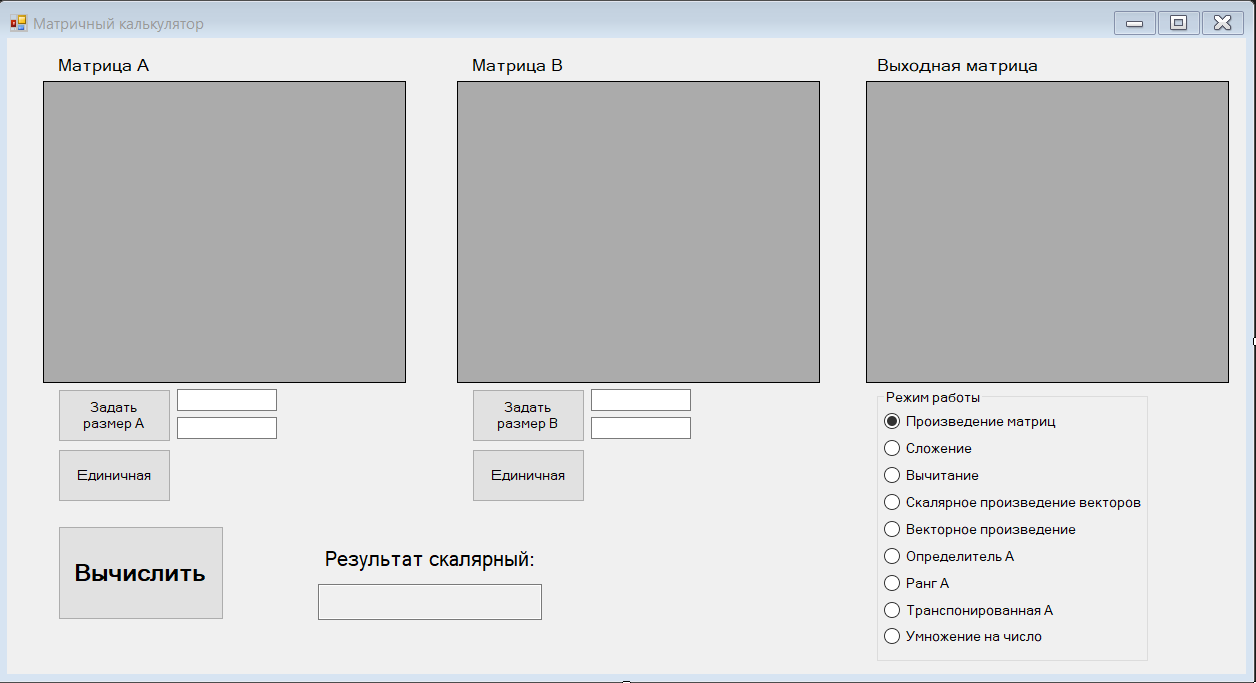
\includegraphics[width=1\linewidth]{lections/img/task6_form.png}
    \caption{Окно приложения «Матричный калькулятор» открытое в конструкторе}
    \label{task6_form}
\end{figure}

\subsection{Таблица с описанием переименованных элементов формы}
Все измененные элементы формы указаны в таблице \ref{task6_attributes}.

\begin{longtable}{|l|l|l|}
\caption{Значения атрибутов элементов в приложении <<Матричный калькулятор>>}\label{task6_attributes}\\
\hline
\textbf{\begin{tabular}[c]{@{}l@{}}Описание элементов\\ формы\end{tabular}}                   & \textbf{\begin{tabular}[c]{@{}l@{}}Список измененных\\ атрибутов\end{tabular}} & \textbf{\begin{tabular}[c]{@{}l@{}}Новое значение\\ атрибута\end{tabular}} \\ \hline
\endfirsthead
%
\endhead
%
Форма MyForm                                                                                  & Text                                                                           & Матричный калькулятор                                                      \\ \hline
\begin{tabular}[c]{@{}l@{}}TextBox ввода количества\\ строк Матрицы А\end{tabular}            & Name                                                                           & set\_size\_A\_lines                                                        \\ \hline
\begin{tabular}[c]{@{}l@{}}TextBox ввода количества\\ столбцов таблицы А\end{tabular}         & Name                                                                           & set\_size\_A\_columns                                                      \\ \hline
\begin{tabular}[c]{@{}l@{}}TextBox ввода количества\\ строк Матрицы B\end{tabular}            & Name                                                                           & set\_size\_B\_lines                                                        \\ \hline
\begin{tabular}[c]{@{}l@{}}TextBox ввода количества\\ столбцов матрицы В\end{tabular}         & Name                                                                           & set\_size\_B\_columns                                                      \\ \hline
\multirow{2}{*}{\begin{tabular}[c]{@{}l@{}}Кнопка "Единичная" под \\ матрицей А\end{tabular}} & Name                                                                           & edbtn                                                                      \\ \cline{2-3} 
                                                                                              & Text                                                                           & Единичная                                                                  \\ \hline
\multirow{2}{*}{\begin{tabular}[c]{@{}l@{}}Кнопка "Единичная" под \\ матрицей B\end{tabular}} & Name                                                                           & edbtnB                                                                     \\ \cline{2-3} 
                                                                                              & Text                                                                           & Единичная                                                                  \\ \hline
\multirow{2}{*}{Кнопка "Вычислить"}                                                           & Name                                                                           & solve                                                                      \\ \cline{2-3} 
                                                                                              & Text                                                                           & Вычислить                                                                  \\ \hline
\begin{tabular}[c]{@{}l@{}}TextBox вывода скалярного\\ ответа\end{tabular}                    & Name                                                                           & output\_scal                                                               \\ \hline
\multirow{2}{*}{Кнопка "Задать размер" А}                                                     & Name                                                                           & set\_size\_A                                                               \\ \cline{2-3} 
                                                                                              & Text                                                                           & Задать размер A                                                            \\ \hline
\multirow{2}{*}{Кнопка "Задать размер" В}                                                     & Name                                                                           & set\_size\_B                                                               \\ \cline{2-3} 
                                                                                              & Text                                                                           & Задать размер B                                                            \\ \hline
\multirow{3}{*}{Таблица Матрица А}                                                            & Name                                                                           & input\_A                                                                   \\ \cline{2-3} 
                                                                                              & AllowUserToAddRows                                                             & False                                                                      \\ \cline{2-3} 
                                                                                              & AllowUserToDeleteRows                                                          & False                                                                      \\ \hline
\multirow{3}{*}{Таблица Матрица B}                                                            & Name                                                                           & input\_B                                                                   \\ \cline{2-3} 
                                                                                              & AllowUserToAddRows                                                             & False                                                                      \\ \cline{2-3} 
                                                                                              & AllowUserToDeleteRows                                                          & False                                                                      \\ \hline
\multirow{4}{*}{Таблица выходной матрицы}                                                     & Name                                                                           & output\_grid                                                               \\ \cline{2-3} 
                                                                                              & AllowUserToAddRows                                                             & False                                                                      \\ \cline{2-3} 
                                                                                              & AllowUserToDeleteRows                                                          & False                                                                      \\ \cline{2-3} 
                                                                                              & ReadOnly                                                                       & True                                                                       \\ \hline
\multirow{2}{*}{\begin{tabular}[c]{@{}l@{}}GroupBox выбора режима\\ работы\end{tabular}}      & Name                                                                           & modes                                                                      \\ \cline{2-3} 
                                                                                              & Text                                                                           & Режим работы                                                               \\ \hline
\multirow{3}{*}{\begin{tabular}[c]{@{}l@{}}RadioButton Произведение\\ матриц\end{tabular}}    & Name                                                                           & mode1\_proiz                                                               \\ \cline{2-3} 
                                                                                              & Text                                                                           & Произведение матриц                                                        \\ \cline{2-3} 
                                                                                              & Checked                                                                        & True                                                                       \\ \hline
\multirow{2}{*}{RadioButton Сложение}                                                         & Name                                                                           & mode2\_sloz                                                                \\ \cline{2-3} 
                                                                                              & Text                                                                           & Сложение                                                                   \\ \hline
\multirow{2}{*}{RadioButton Вычитание}                                                        & Name                                                                           & mode3\_sub                                                                 \\ \cline{2-3} 
                                                                                              & Text                                                                           & Вычитание                                                                  \\ \hline
\multirow{2}{*}{\begin{tabular}[c]{@{}l@{}}RadioButton Скалярное\\ произведение\end{tabular}} & Name                                                                           & mode4\_skalproz                                                            \\ \cline{2-3} 
                                                                                              & Text                                                                           & \begin{tabular}[c]{@{}l@{}}Скалярное произведение\\ векторов\end{tabular}  \\ \hline
\multirow{2}{*}{\begin{tabular}[c]{@{}l@{}}RadioButton векторное\\ произведение\end{tabular}} & Name                                                                           & mode5\_vectproz                                                            \\ \cline{2-3} 
                                                                                              & Text                                                                           & Векторное произведение                                                     \\ \hline
\multirow{2}{*}{RadioButton Определитель А}                                                   & Name                                                                           & mode6\_oprA                                                                \\ \cline{2-3} 
                                                                                              & Text                                                                           & Определитель А                                                             \\ \hline
\multirow{2}{*}{RadioButton Ранг А}                                                           & Name                                                                           & mode7\_rankA                                                               \\ \cline{2-3} 
                                                                                              & Text                                                                           & Ранг А                                                                     \\ \hline
\multirow{2}{*}{\begin{tabular}[c]{@{}l@{}}RadioButton\\ Транспонированная А\end{tabular}}    & Name                                                                           & mode8\_tranA                                                               \\ \cline{2-3} 
                                                                                              & Text                                                                           & Транспонированная А                                                        \\ \hline
\multirow{2}{*}{\begin{tabular}[c]{@{}l@{}}RadioButton Умножение\\ на число\end{tabular}}     & Name                                                                           & mode9\_numproz                                                             \\ \cline{2-3} 
                                                                                              & Text                                                                           & Умножение на число                                                         \\ \hline
\end{longtable}


\subsection{Примеры правильной и неправильной работы}
После запуска программы на экране появляется окно на рисунке \ref{task6_launch1}.
\begin{figure}[H]
    \centering
    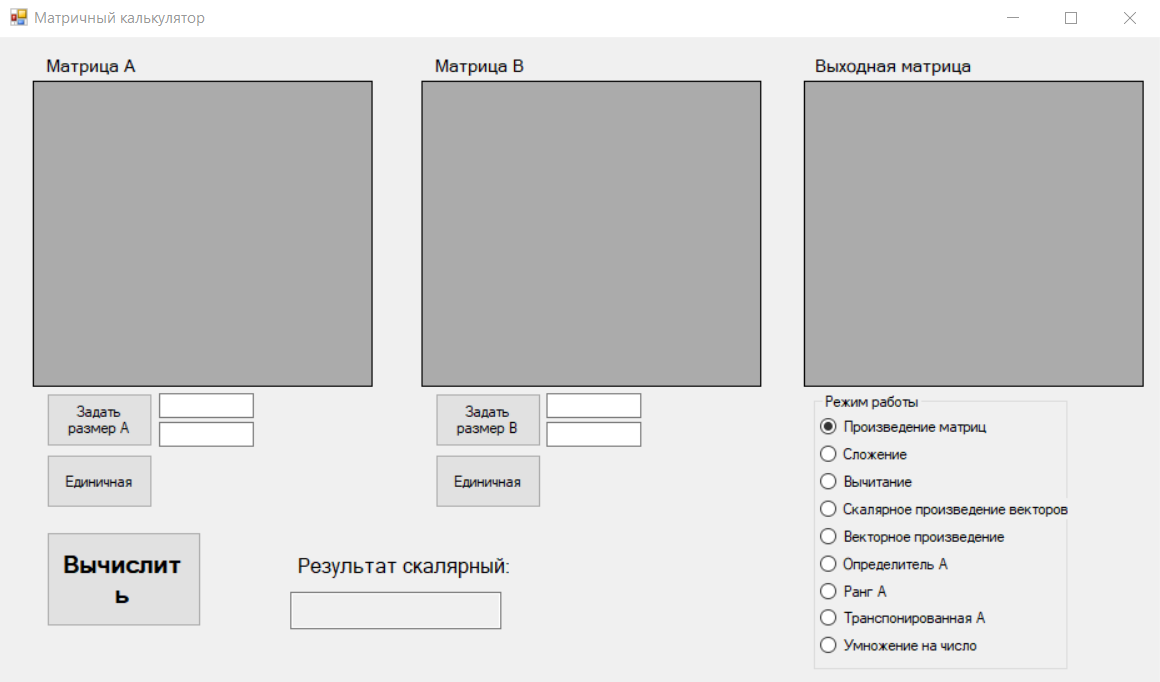
\includegraphics[width=1\linewidth]{lections/img/task6_launch1.png}
    \caption{Запуск программы}
    \label{task6_launch1}
\end{figure}

После ввода двух матриц и нажатии на кнопку "Вычислить" (на рисунке \ref{task6_launch2}).

\begin{figure}[H]
    \centering
    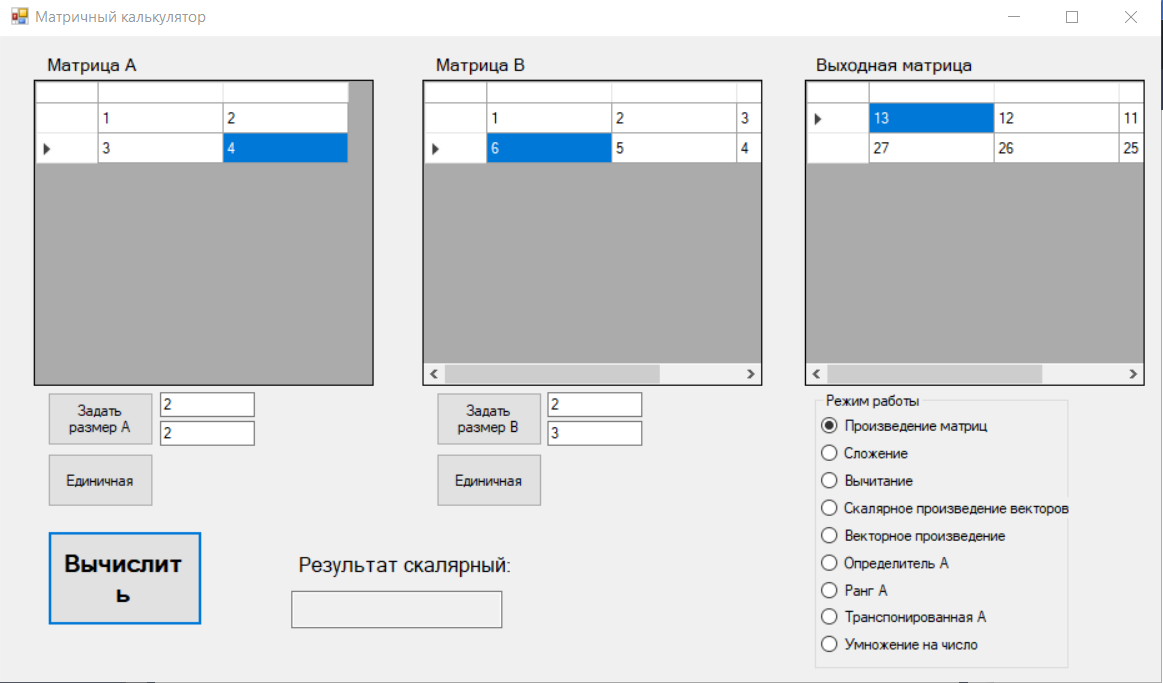
\includegraphics[width=1\linewidth]{lections/img/task6_launch2.png}
    \caption{Произведение матриц}
    \label{task6_launch2}
\end{figure}

При попытке ввода не числа в таблицу, программа выведет ошибку (на рисунке \ref{task6_launch3})
\begin{figure}[H]
    \centering
    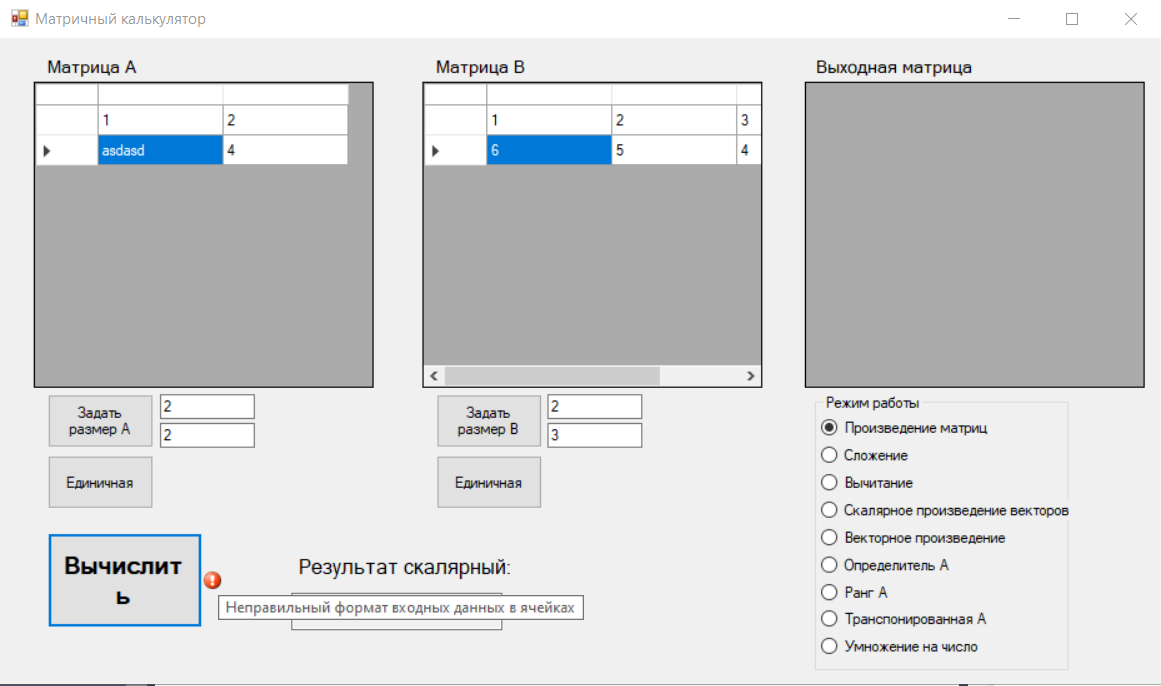
\includegraphics[width=1\linewidth]{lections/img/task6_launch3.png}
    \caption{Ошибка формата ввода}
    \label{task6_launch3}
\end{figure}


\subsection{Примеры исходного кода}


Функция cоздания единичной матрицы B.
\begin{minted}[style=bw,
 linenos=true,
 breaklines=true,
 numbersep=5pt,
 tabsize=2,
 fontsize=\small,
 bgcolor=white]{cpp}
private: System::Void edbtnB_Click(System::Object^ sender, System::EventArgs^ e) {
	int line_count = this->input_B->RowCount;
	int column_count = this->input_B->ColumnCount;
	try {
		if (line_count != column_count) throw gcnew Exception("Матрица не квадратная");
		for (int i = 0; i < line_count; i++) {
			for (int j = 0; j < line_count; j++) {
				if (i == j) this->input_B->Rows[i]->Cells[j]->Value = 1;
				else this->input_B->Rows[i]->Cells[j]->Value = 0;
			}
		}
	}
	catch (Exception^ e) {
		this->errorProvider1->SetError(this->solve, e->Message);
	}
}
\end{minted}
Другие фрагменты кода расположены в приложении \ref{app:matrix}.
\sectionbreak
\section{Использование коллекций}

\subsection{Условие задания}

Разработать приложение в соответствии со своим вариантом. Номер варианта выдает преподаватель. 

Приложение должно содержать следующие пункты:

\begin{enumerate}
    \item Заголовок формы должен отражать суть задания.
    \item Все элементы формы должны быть внятно подписаны (кнопки подписаны, у тестового поля должно быть написано, для чего оно нужно и т. д.)
    \item В коде должны быть комментарии и отступы (код должен быть легко читаем).
    \item В коде программы все элементы формы должны быть переименованы (btnName -  для кнопок, lblName - для ссылок, txtName - для текстового поля и т. д.) Наименования должны быть понятными.
    \item Должна быть возможность для ввода и вывода первоначальных данных.
    \item Должна быть возможность для вставки и удаления одного элемента.
    \item Должны использоваться коллекции.
    \item Ответы на задания должны быть в разных полях.
    \item Если нет данных для выполнения задания, выводить соответствующие данные.
    \item Для графов использовать список смежности.
\end{enumerate}

\textbf{Вариант 7.} Создать стек, состоящий из целых чисел. Предусмотреть возможность создания стека из набора чисел, добавления одного элемента (функция push), удаления одного элемента (функция pop), вывода результата на экран, удаления всех элементов с помощью кнопок. Найти максимальный нечетный элемент. Получить новый стек, удалив все нечетные элементы.


\subsection{Вид формы в конструкторе}



Для реализации стека создано окно приложения, содержащее пять элементов TextBox, три элемента Label, пять элементов Button и один элемент ErrorProvider для обработки ошибок. Вид окна представлен на рисунке \ref{task7_form} \cite{chang2021analysis}.
\begin{figure}[H]
    \centering
    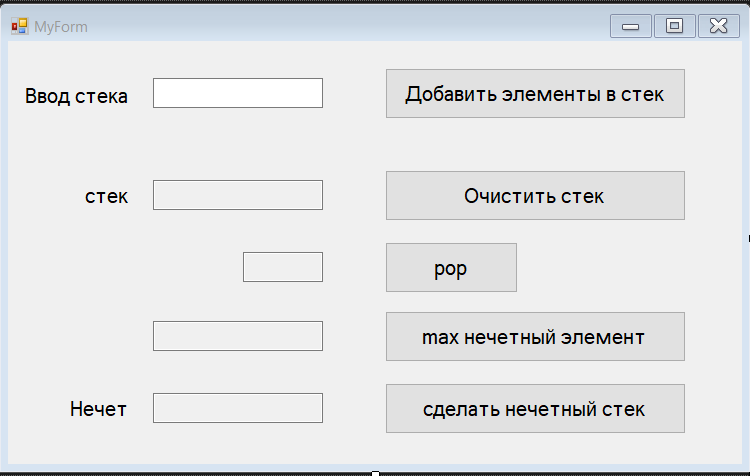
\includegraphics[width=1\linewidth]{lections/img/task7_form.png}
    \caption{Окно приложения «Матричный калькулятор» открытое в конструкторе}
    \label{task7_form}
\end{figure}



\subsection{Таблица с описанием переименованных элементов формы}
Все измененные элементы формы указаны в таблице \ref{task7_attributes}.


\begin{longtable}{|l|l|l|}
\caption{Значения атрибутов элементов в приложении <<Работа с коллекциями>>}\label{task7_attributes}\\
\hline
\textbf{\begin{tabular}[c]{@{}l@{}}Описание элементов\\ формы\end{tabular}}                                & \textbf{\begin{tabular}[c]{@{}l@{}}Список измененных\\ атрибутов\end{tabular}} & \textbf{\begin{tabular}[c]{@{}l@{}}Новое значение\\ атрибута\end{tabular}} \\ \hline
\endfirsthead
%
\endhead
%
Форма MyForm                                                                                               & Text                                                                           & Работа с коллекциями                                                       \\ \hline
TextBox ввода стека                                                                                        & Name                                                                           & input\_stack                                                               \\ \hline
\multirow{2}{*}{TextBox вывода стека}                                                                      & Name                                                                           & output                                                                     \\ \cline{2-3} 
                                                                                                           & ReadOnly                                                                       & True                                                                       \\ \hline
\multirow{2}{*}{\begin{tabular}[c]{@{}l@{}}TextBox вывода pop\\ элемента\end{tabular}}                     & Name                                                                           & pop\_out                                                                   \\ \cline{2-3} 
                                                                                                           & ReadOnly                                                                       & True                                                                       \\ \hline
\multirow{2}{*}{\begin{tabular}[c]{@{}l@{}}TextBox вывода максимального\\ нечетного элемента\end{tabular}} & Name                                                                           & max\_nech                                                                  \\ \cline{2-3} 
                                                                                                           & ReadOnly                                                                       & True                                                                       \\ \hline
\multirow{2}{*}{\begin{tabular}[c]{@{}l@{}}TextBox вывода стека из\\ нечетных элементов\end{tabular}}      & Name                                                                           & nech\_stack                                                                \\ \cline{2-3} 
                                                                                                           & ReadOnly                                                                       & True                                                                       \\ \hline
\multirow{2}{*}{\begin{tabular}[c]{@{}l@{}}Кнопка "Добавить элементы\\ в стек"\end{tabular}}               & Name                                                                           & create\_stack                                                              \\ \cline{2-3} 
                                                                                                           & Text                                                                           & \begin{tabular}[c]{@{}l@{}}Добавить элементы в\\ стек\end{tabular}         \\ \hline
\multirow{2}{*}{Кнопка "Очистить стек"}                                                                    & Name                                                                           & clear\_stack                                                               \\ \cline{2-3} 
                                                                                                           & Text                                                                           & Очистить стек                                                              \\ \hline
\multirow{2}{*}{Кнопка "pop"}                                                                              & Name                                                                           & pop\_stack                                                                 \\ \cline{2-3} 
                                                                                                           & Text                                                                           & pop                                                                        \\ \hline
\multirow{2}{*}{\begin{tabular}[c]{@{}l@{}}Кнопка "max нечетный \\ элемент"\end{tabular}}                  & Name                                                                           & max\_nech\_btn                                                             \\ \cline{2-3} 
                                                                                                           & Text                                                                           & max нечетный элемент                                                       \\ \hline
\multirow{2}{*}{\begin{tabular}[c]{@{}l@{}}Кнопка "Сделать нечетный\\ стек"\end{tabular}}                  & Name                                                                           & nech\_stack\_btn                                                           \\ \cline{2-3} 
                                                                                                           & Text                                                                           & сделать нечетный стек                                                      \\ \hline
\end{longtable}


\subsection{Примеры правильной и неправильной работы}
После запуска программы на экране появляется окно на рисунке \ref{task7_launch1}.
\begin{figure}[H]
    \centering
    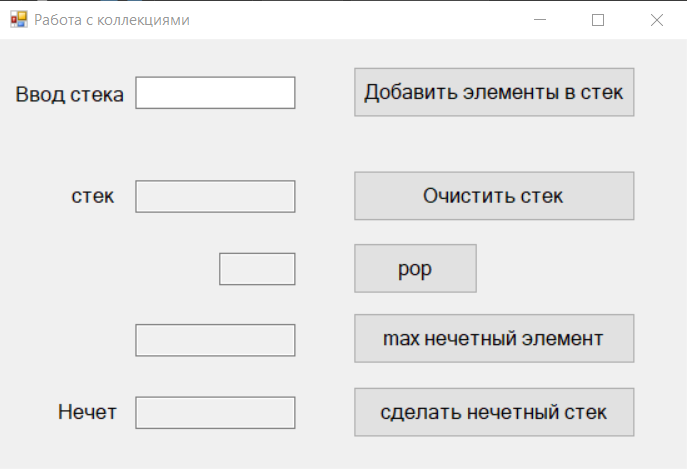
\includegraphics[width=0.8\linewidth]{lections/img/task7_launch1.png}
    \caption{Запуск программы}
    \label{task7_launch1}
\end{figure}

После ввода поле целых чисел через пробел и нажатии на кнопку "Добавить элементы в стек" (на рисунке \ref{task7_launch2}).

\begin{figure}[H]
    \centering
    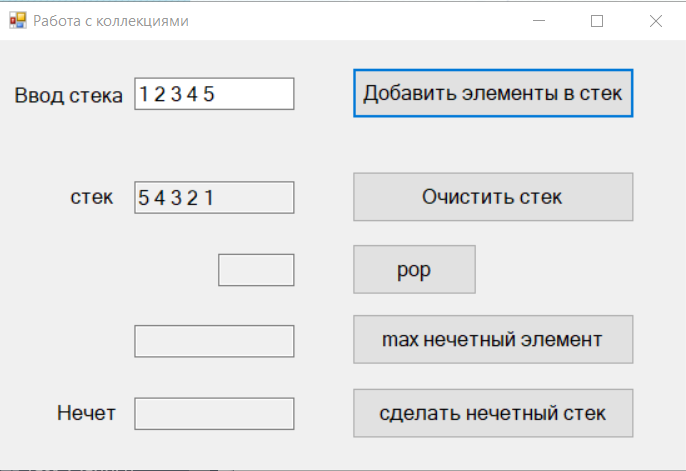
\includegraphics[width=0.8\linewidth]{lections/img/task7_launch2.png}
    \caption{Ввод стека}
    \label{task7_launch2}
\end{figure}

При попытке ввода не числа в поле, программа выведет ошибку (на рисунке \ref{task7_launch3})
\begin{figure}[H]
    \centering
    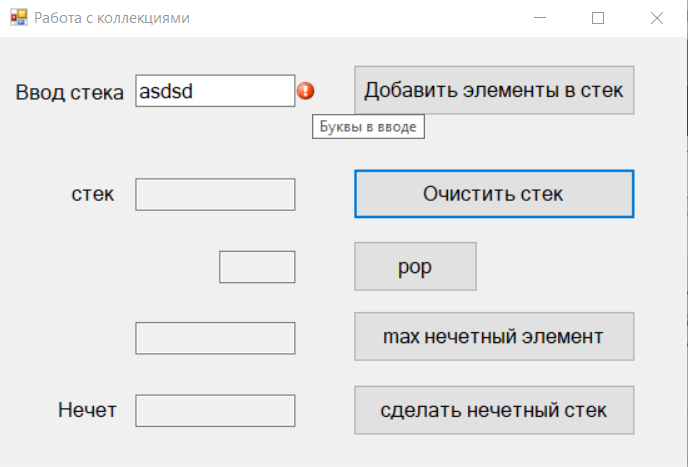
\includegraphics[width=0.8\linewidth]{lections/img/task7_launch3.png}
    \caption{Ошибка формата ввода}
    \label{task7_launch3}
\end{figure}



\subsection{Примеры исходного кода}


Функция очистки стека.
\begin{minted}[style=bw,
 linenos=true,
 breaklines=true,
 numbersep=5pt,
 tabsize=2,
 fontsize=\small,
 bgcolor=white]{cpp}
private: System::Void stack_out() {
	System::Collections::Generic::Stack<int> buf; //вспомогательный стек
	System::String^ str2 = "";
	while (s.Count) {//пока стек не пуст
		buf.Push(s.Peek()); //записываем во вспомогательный стек первый элемент
		str2 += System::Convert::ToString(s.Peek()) + " "; //записываем первый элемент в строку
		s.Pop(); //удаляем первый элемент из стека


	}
	while (buf.Count) { //пока вспомогательный стек не пуст
		s.Push(buf.Peek()); //записываем в основной стек первый элемент вспомогательного
		buf.Pop(); //удаляем из стека первый элемент

	}

	this->output->Text = str2; //записываем результат в строку
}
\end{minted}
Другие фрагменты кода расположены в приложении \ref{app:collections}.
\sectionbreak
\section{Работа с файлами}

\subsection{Условие задания}

Разработать приложение для своего варианта. 

Приложение должно содержать следующие компоненты:

\begin{enumerate}
    \item Заголовок формы должен отражать суть задания.
    \item Все элементы формы должны быть внятно подписаны (кнопки подписаны, у тестового поля должно быть написано, для чего оно нужно и т. д.)
    \item Структура представляет собой таблицу DataGridView, в ячейках которой записаны данные разных типов. 
    \item Предусмотреть кнопки: 
    \begin{itemize}
        \item считывание данных из файла и запись данных в таблицу (предполагается, что в файле данные корректные); 
        \item возможность добавлять и удалять строки в таблице, соответственно, вводить данные вручную.
        \item  запись в файл всех данных. Проверять корректность ввода данных: даты должны быть реальные, номер телефона состоять из цифр и, может быть, знак тире, оценки студентов - от 2 до 5. Все остальное можно не проверять. Если есть срок пребывания, дата прибытия и дата отбытия, то срок пребывания должен быть равен разнице между датой отбытия и датой прибытия.
        \item запись в файл данных по определенному критерию. Критерий можно вводить вручную через TextBox или выбирать c помощью Radiobox и т. д. Запись в файл должна быть такой, чтобы этот файл можно было открыть в приложении.
        \item запись данных по определенному критерию в новую таблицу. При выборе другого критерия старая таблица должна удаляться.
    \end{itemize}
    \item При неправильном вводе каких-либо данных таблица выбранных данных должна очищаться. 
    \item В коде должны быть комментарии и отступы (код должен быть легко читаем).
\end{enumerate}

\textbf{Вариант 11.} Создать таблицу \texttt{Travel}, содержащую следующие поля: Фамилия, имя, отчество туриста, название гостиницы, срок пребывания, дата приезда, дата отъезда. Выполнить следующие действия: считать из файла и вывести на экран данные о всех туристах, в другой файл вывести данные о туристах, приезжающих в данный день.

\subsection{Вид формы в конструкторе}


Создано окно приложения, содержащее один элемент TextBox, один элемент Label, шесть элементов Button, два элемента gridview,один элемент ErrorProvider для обработки ошибок и saveFileDialog и openFileDialog для работы с файлами. Вид окна представлен на рисунке \ref{task8_form} \cite{gladstone2022building}\cite{kaiser2022c++}.
\begin{figure}[H]
    \centering
    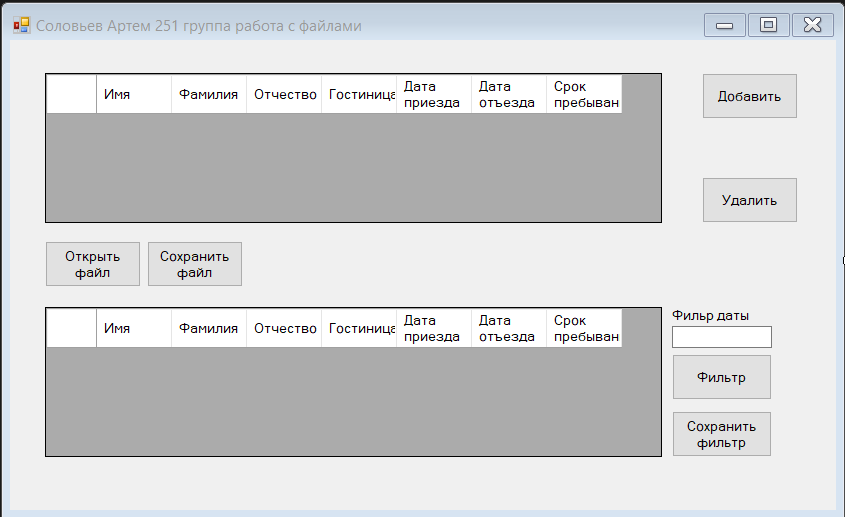
\includegraphics[width=1\linewidth]{lections/img/task8_form.png}
    \caption{Окно приложения «Матричный калькулятор» открытое в конструкторе}
    \label{task8_form}
\end{figure}


\subsection{Таблица с описанием переименованных элементов формы}
Все измененные элементы формы указаны в таблице \ref{task8_attributes}.


\begin{longtable}{|l|l|l|}
\caption{Значения атрибутов элементов в приложении <<Работа с файлами>>}\label{task8_attributes}\\
\hline
\textbf{\begin{tabular}[c]{@{}l@{}}Описание элементов\\ формы\end{tabular}}                         & \textbf{\begin{tabular}[c]{@{}l@{}}Список измененных\\ атрибутов\end{tabular}} & \textbf{\begin{tabular}[c]{@{}l@{}}Новое значение\\ атрибута\end{tabular}}             \\ \hline
\endfirsthead
%
\endhead
%
Форма MyForm                                                                                        & Text                                                                           & \begin{tabular}[c]{@{}l@{}}Соловьев Артем 251\\ группа работа с\\ файлами\end{tabular} \\ \hline
TextBox фильтра даты                                                                                & Name                                                                           & FilterDate                                                                             \\ \hline
\multirow{2}{*}{Кнопка "Добавить"}                                                                  & Name                                                                           & AddRow                                                                                 \\ \cline{2-3} 
                                                                                                    & Text                                                                           & Добавить                                                                               \\ \hline
\multirow{2}{*}{Кнопка "Удалить"}                                                                   & Name                                                                           & DeleteRow                                                                              \\ \cline{2-3} 
                                                                                                    & Text                                                                           & Удалить                                                                                \\ \hline
\multirow{2}{*}{Кнопка открытия файла}                                                              & Name                                                                           & FileOpen                                                                               \\ \cline{2-3} 
                                                                                                    & Text                                                                           & Открыть файл                                                                           \\ \hline
\multirow{2}{*}{Кнопка сохранения файла}                                                            & Name                                                                           & FileSave                                                                               \\ \cline{2-3} 
                                                                                                    & Text                                                                           & Сохранить файл                                                                         \\ \hline
\multirow{2}{*}{Кнопка фильтр даты}                                                                 & Name                                                                           & FilterBtn                                                                              \\ \cline{2-3} 
                                                                                                    & Text                                                                           & Фильтр                                                                                 \\ \hline
\multirow{2}{*}{\begin{tabular}[c]{@{}l@{}}Кнопка сохранить\\ отфильтрованную таблицу\end{tabular}} & Name                                                                           & FileSaveFilter                                                                         \\ \cline{2-3} 
                                                                                                    & Text                                                                           & Сохранить фильтр                                                                       \\ \hline
\multirow{2}{*}{Таблица постояльцев}                                                                & Name                                                                           & MainTable                                                                              \\ \cline{2-3} 
                                                                                                    & AllowUserToAddRows                                                             & False                                                                                  \\ \hline
\multirow{4}{*}{\begin{tabular}[c]{@{}l@{}}Таблица постояльцев\\ (отфильтрованная)\end{tabular}}    & Name                                                                           & FilteredTable                                                                          \\ \cline{2-3} 
                                                                                                    & AllowUserToAddRows                                                             & False                                                                                  \\ \cline{2-3} 
                                                                                                    & AllowUserToDeleteRows                                                          & False                                                                                  \\ \cline{2-3} 
                                                                                                    & ReadOnly                                                                       & True                                                                                   \\ \hline

\end{longtable}


\subsection{Примеры правильной и неправильной работы}
После запуска программы на экране появляется окно на рисунке \ref{task8_launch1}.
\begin{figure}[H]
    \centering
    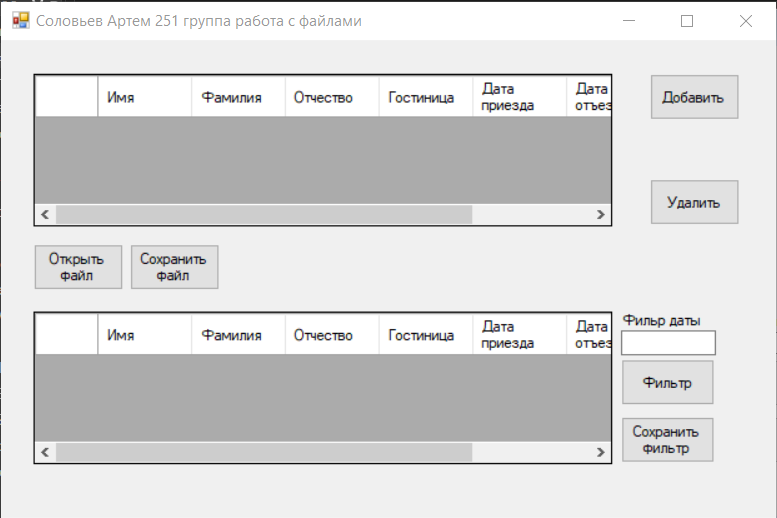
\includegraphics[width=0.8\linewidth]{lections/img/task8_launch1.png}
    \caption{Запуск программы}
    \label{task8_launch1}
\end{figure}

После ввода данных постояльцев, даты в фильтр даты и нажатии на кнопку "Фильтр" (на рисунке \ref{task8_launch2}).

\begin{figure}[H]
    \centering
    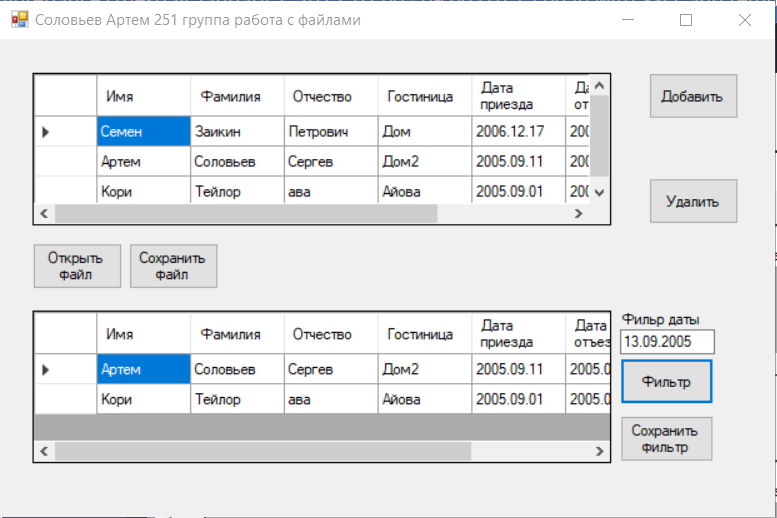
\includegraphics[width=0.8\linewidth]{lections/img/task8_launch2.png}
    \caption{Отфильтрованная таблица}
    \label{task8_launch2}
\end{figure}

При попытке ввода не даты в поле, программа выведет ошибку (на рисунке \ref{task8_launch3})
\begin{figure}[H]
    \centering
    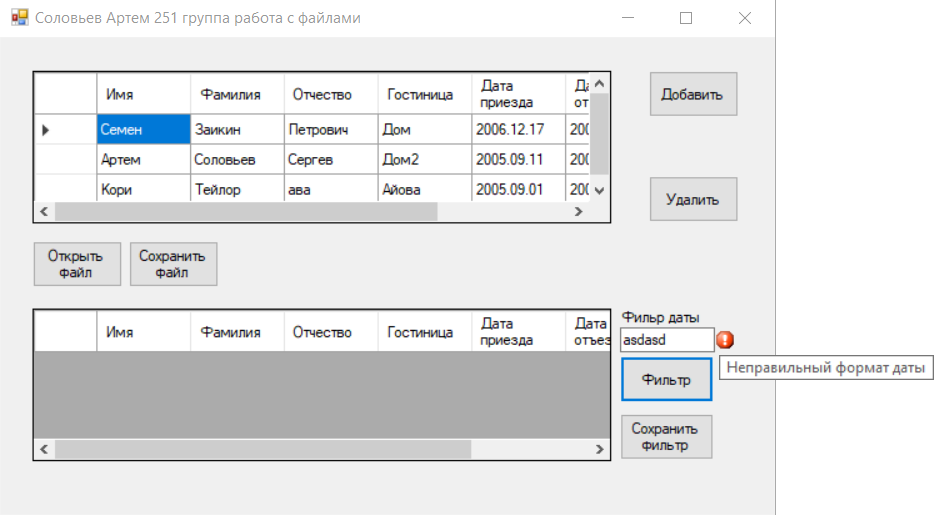
\includegraphics[width=1\linewidth]{lections/img/task8_launch3.png}
    \caption{Ошибка формата ввода}
    \label{task8_launch3}
\end{figure}


\subsection{Примеры исходного кода}


Функция удаления строки таблицы.
\begin{minted}[style=bw,
 linenos=true,
 breaklines=true,
 numbersep=5pt,
 tabsize=2,
 fontsize=\small,
 bgcolor=white]{cpp}
private: System::Void DeleteRow_Click(System::Object^ sender, System::EventArgs^ e) {
	this->errorProvider1->Clear();
	if (this->MainTable->RowCount == 0) {
		this->errorProvider1->SetError(DeleteRow, "Нельзя убрать строку, которой нет");
		return;
	}
	int i = this->MainTable->CurrentRow->Index;
	this->MainTable->Rows->Remove(this->MainTable->Rows[i]);
}
\end{minted}
Другие фрагменты кода расположены в приложении \ref{app:files}.

\sectionbreak
\section{Приложение ТЕСТ}

\subsection{Условие задания}

Создать приложение для проведения тестирования.

Должно содержать:
\begin{enumerate}
    \item Набор вопросов по какой-то теме (и вопросы и ответы должны быть реальные) -не менее 10
    \item Вопросы должны выбираться случайным образом.
    \item Вопросы должны быть нескольких типов - "Да/нет", Выбор одного ответа, Выбор нескольких ответов, Короткий ответ.
    \item Необходимо создать сообщения для правильного и неправильного ответа (Молодец, Не правильно и т.д.)
    \item Необходимо подсчитать количество правильных ответов и вывести результат.
\end{enumerate}

\subsection{Вид формы в конструкторе}


Создано две формы приложения, содержащие три элемента TextBox, три элемента Label, один элемент Button, один элемент ErrorProvider для обработки ошибок и один элемент groupBox с четыремя элементами checkbox. Вид окна вопроса представлен на рисунке \ref{task9_form1} \cite{зиборов2011ms}.
\begin{figure}[H]
    \centering
    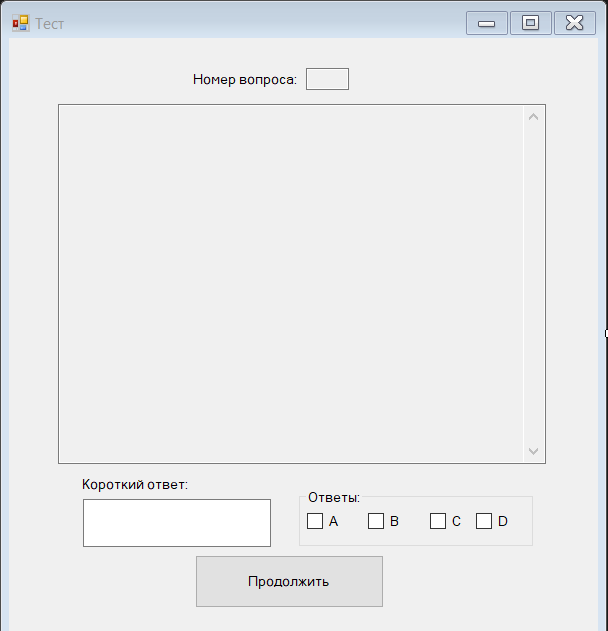
\includegraphics[width=0.8\linewidth]{lections/img/task9_form1.png}
    \caption{Окно вопросов приложения «Тест» открытое в конструкторе}
    \label{task9_form1}
\end{figure}

Вид окна результата представлен на рисунке \ref{task9_form2}.
\begin{figure}[H]
    \centering
    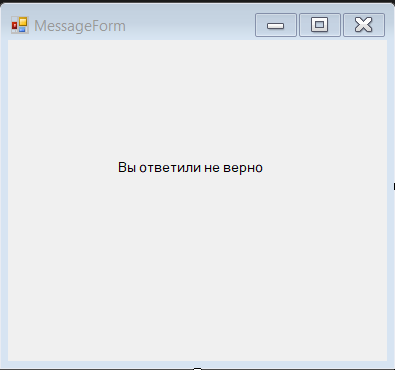
\includegraphics[width=0.5\linewidth]{lections/img/task9_form2.png}
    \caption{Окно результата приложения «Тест» открытое в конструкторе}
    \label{task9_form2}
\end{figure}


\subsection{Таблица с описанием переименованных элементов формы}
Все измененные элементы формы указаны в таблице \ref{task9_attributes}.

\begin{longtable}{|l|l|l|}
\caption{Значения атрибутов элементов в приложении <<Тест>>}\label{task9_attributes}\\
\hline
\textbf{\begin{tabular}[c]{@{}l@{}}Описание элементов\\ формы\end{tabular}}           & \textbf{\begin{tabular}[c]{@{}l@{}}Список измененных\\ атрибутов\end{tabular}} & \textbf{\begin{tabular}[c]{@{}l@{}}Новое значение\\ атрибута\end{tabular}} \\ \hline
\endfirsthead
%
\endhead
%
Форма MyForm                                                                          & Text                                                                           & Тест                                                                       \\ \hline
\multirow{2}{*}{TextBox номера вопроса}                                               & Name                                                                           & countBox                                                                   \\ \cline{2-3} 
                                                                                      & ReadOnly                                                                       & True                                                                       \\ \hline
\multirow{2}{*}{TextBox короткого ответа}                                             & Name                                                                           & shortAns                                                                   \\ \cline{2-3} 
                                                                                      & Multiline                                                                      & True                                                                       \\ \hline
\multirow{3}{*}{TextBox текста вопроса}                                               & Name                                                                           & questBox                                                                   \\ \cline{2-3} 
                                                                                      & Multiline                                                                      & True                                                                       \\ \cline{2-3} 
                                                                                      & ReadOnly                                                                       & True                                                                       \\ \hline
\multirow{2}{*}{Кнопка ответа}                                                        & Name                                                                           & act                                                                        \\ \cline{2-3} 
                                                                                      & Text                                                                           & Продолжить                                                                 \\ \hline
\multirow{2}{*}{\begin{tabular}[c]{@{}l@{}}GroupBox вариантов\\ ответа\end{tabular}}  & Name                                                                           & answerGroup                                                                \\ \cline{2-3} 
                                                                                      & Text                                                                           & Ответы:                                                                    \\ \hline
\multirow{2}{*}{\begin{tabular}[c]{@{}l@{}}CheckBox варианта ответа\\ А\end{tabular}} & Name                                                                           & answerA                                                                    \\ \cline{2-3} 
                                                                                      & Text                                                                           & A                                                                          \\ \hline
\multirow{2}{*}{\begin{tabular}[c]{@{}l@{}}CheckBox варианта ответа\\ B\end{tabular}} & Name                                                                           & answerB                                                                    \\ \cline{2-3} 
                                                                                      & Text                                                                           & B                                                                          \\ \hline
\multirow{2}{*}{\begin{tabular}[c]{@{}l@{}}CheckBox варианта ответа\\ C\end{tabular}} & Name                                                                           & answerC                                                                    \\ \cline{2-3} 
                                                                                      & Text                                                                           & C                                                                          \\ \hline
\multirow{2}{*}{\begin{tabular}[c]{@{}l@{}}CheckBox варианта ответа\\ D\end{tabular}} & Name                                                                           & answerD                                                                    \\ \cline{2-3} 
                                                                                      & Text                                                                           & D                                                                          \\ \hline

\end{longtable}


\subsection{Примеры правильной и неправильной работы}
После запуска программы на экране появляется окно на рисунке \ref{task9_launch1}.
\begin{figure}[H]
    \centering
    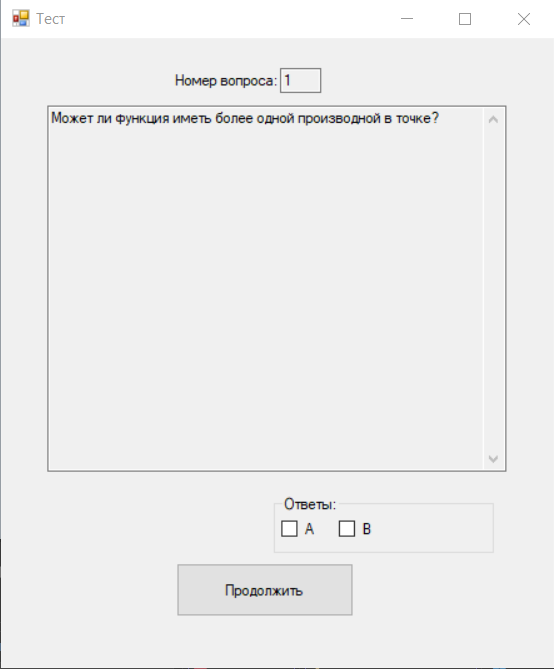
\includegraphics[width=0.8\linewidth]{lections/img/task9_launch1.png}
    \caption{Запуск программы}
    \label{task9_launch1}
\end{figure}

После выбора варианта ответа и нажатия кнопки "Продолжить" ( на рисунке \ref{task9_launch2}).

\begin{figure}[H]
    \centering
    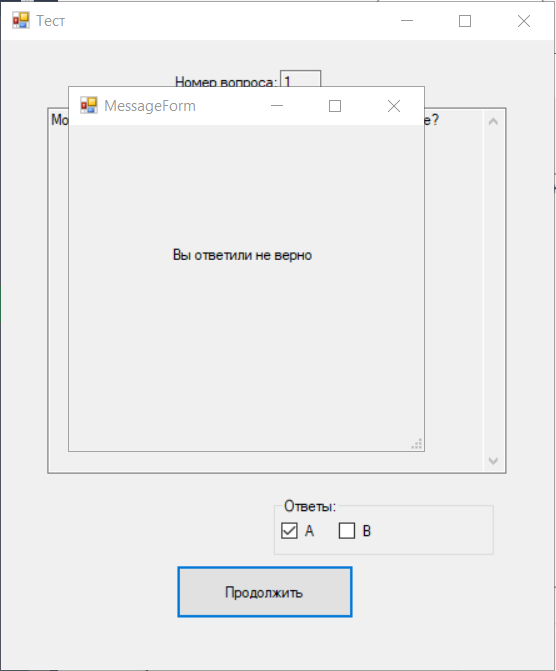
\includegraphics[width=0.8\linewidth]{lections/img/task9_launch2.png}
    \caption{Отфильтрованная таблица}
    \label{task9_launch2}
\end{figure}

При выбрать одновременно "Да" и "Нет" вылазит ошибка (на рисунке \ref{task9_launch3})
\begin{figure}[H]
    \centering
    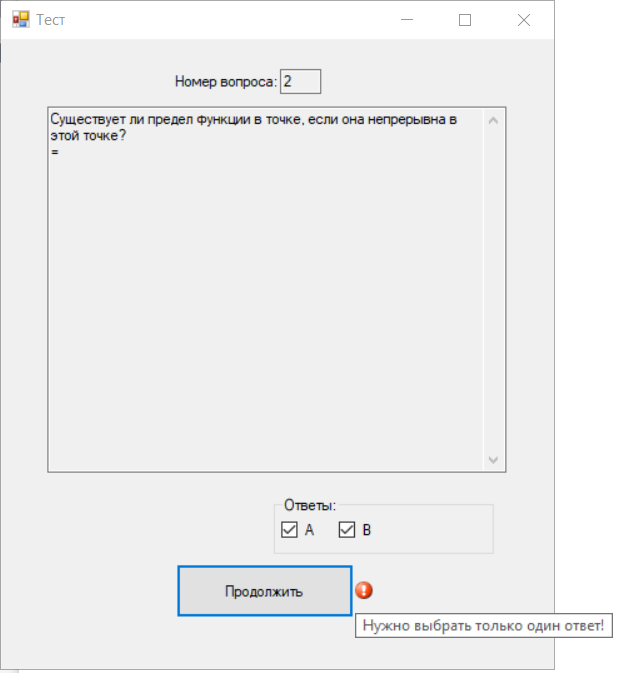
\includegraphics[width=0.8\linewidth]{lections/img/task9_launch3.png}
    \caption{Ошибка формата ввода}
    \label{task9_launch3}
\end{figure}

\subsection{Примеры исходного кода}


Функция считывания вопроса из вектора.
\begin{minted}[style=bw,
 linenos=true,
 breaklines=true,
 numbersep=5pt,
 tabsize=2,
 fontsize=\small,
 bgcolor=white]{cpp}
std::string ReadAnswer() {
	int i = RandIndex->at(iter);
	Quest temp = Questions->at(i);
	if (temp.getType() == "ДаНет") {
		return YesNoRead();
	}
	else if (temp.getType() == "ОдинОтвет") {
		return OneAnswerRead();
	}
	else if (temp.getType() == "НесколькоОтветов") {
		return SomeAnswersRead();
	}
	else {
		return ShortAnswerRead();
	}

}
\end{minted}
Другие фрагменты кода расположены в приложении \ref{app:test}.
\sectionbreak

\conclusion

В ходе практики было реализовано несколько приложений в среде Microsoft Visual Studio с целью закрепления навыков построения оконного интерфейса и программирования с использованием C++/CLI.

На практике разработаны приложения, содержащие такие элементы интерфейса, как TextBox, Label, Button, DataGridView, OpenFileDialog, SaveFileDialog, ErrorProvider.

Было освоено динамическое создание элементов формы в процессе выполнения программы, изучены виды панелей и способы размещения элементов в них. Также были применены навыки программирования на основе обратных вызовов при обработке событий формы.

\sectionbreak

\nocite{*}
\bibliographystyle{ugost2003}
\bibliography{lib}

\appendix
\section{Фрагменты кода программы <<Вычисление факториала>>}
\label{app:factorial}
Функция вычисления факториала:

\begin{minted}[style=bw,
 linenos=true,
 breaklines=true,
 numbersep=5pt,
 tabsize=2,
 fontsize=\small,
 bgcolor=white]{cpp}
long long fact(long long N) {
	if (N < 0) //отрицательное число
		return -1;
	else if (N == 0 || N == 1) // 0! = 1
		return 1;
	else
		return N * fact(N - 1); //n! = n * (n - 1)!
}
\end{minted}
\section{Фрагменты кода программы <<Простые вычисления>>}
\label{app:simple_calculations}

Функция, при нажатии на кнопку <<Вычислить>>.
\begin{minted}[style=bw,
 linenos=true,
 breaklines=true,
 numbersep=5pt,
 tabsize=2,
 fontsize=\small,
 bgcolor=white]{cpp}
private: System::Void solvebtn_Click(System::Object^ sender, System::EventArgs^ e) {
	this->output->Text = ""; // Стираем поле вывода

	errors->SetError(x_input, String::Empty); // обнуляем ошибки
	errors->SetError(y_input, String::Empty);

	Int64 x, y; // Переменные для считывания полей ввода
	double result; // переменная для записи результата

	bool result_x = Int64::TryParse(this->x_input->Text, x); // записываем из полей ввода в соответствующие переменные
	bool result_y = Int64::TryParse(this->y_input->Text, y); // и проверяем на успешность выполнения парсинга

	if (!result_x) { // если неудачно
		errors->SetError(x_input, "Введено не целое число");
	}
	if (!result_y) {
		errors->SetError(y_input, "Введено не целое число");
	}
	if (result_x && result_y) { // если удачно
		if (x * x - y == 0) { // проверка на ОДЗ
			this->output->Text = "Деление на ноль";
		}
		else {
			result = (1.0) * ((x + y) * (x + y) - x * x * x) / (std::abs(x * x - y)); //Считаем
			this->output->Text = System::Convert::ToString(result); //Записываем результат
		}
	}
}
\end{minted}

\section{Фрагменты кода программы <<Рекурсивные вычисления>>}
\label{app:recursive_calculations}


Функция обработки нажатия на кнопку <<Вычислить>>.
\begin{minted}[style=bw,
 linenos=true,
 breaklines=true,
 numbersep=5pt,
 tabsize=2,
 fontsize=\small,
 bgcolor=white]{cpp}
private: System::Void Solve_Click(System::Object^ sender, System::EventArgs^ e) {
	ClearAll();
	long long n, m, A;
	bool result_n = Int64::TryParse(this->n_input->Text, n);
	bool result_m = Int64::TryParse(this->m_input->Text, m);
	if (!result_n) {
		errorProvider1->SetError(this->n_input, "Неправильно введено число n.");
	}
	if (!result_m) {
		errorProvider1->SetError(this->m_input, "Неправильно введено число m.");
	}
	if (result_m && result_n) {

		if (n > m) {
			this->Output->Text = "Ошибка: n > m";
		}
		else {
			if (n < 1) {
				this->Output->Text = "" + "Ошибка: n < 1 "+ System::Environment::NewLine;
			}
			if (m < 1) {
				this->Output->Text += "Ошибка: m < 1\n";
			}
			if (n >= 1 && m >= 1) {
				this->Output->Text = "Количество различных размещений из n в m равно: " + System::Convert::ToString(per(n, m));
			}
		}
	}
}
\end{minted}
\section{Фрагменты кода программы <<Обработка табличных данных. Часть 1>>}
\label{app:table_data}

Функция обработки нажатия на кнопку "Минимум"
\begin{minted}[style=bw,
 linenos=true,
 breaklines=true,
 numbersep=5pt,
 tabsize=2,
 fontsize=\small,
 bgcolor=white]{cpp}
private: System::Void min_btn_Click(System::Object^ sender, System::EventArgs^ e) {
	long long y, maxel = 1e9;
	bool found_chet = false;
	for (int i = 0; i < this->mas_grid->RowCount; i++) {
		bool result = Int64::TryParse(this->mas_grid->Rows[i]->Cells[0]->Value->ToString(), y);
		if (y % 2 == 0) {
			found_chet = true;
			maxel = (y < maxel) ? y : maxel;
		}
	}
	if (found_chet)	this->chet_box->Text = System::Convert::ToString(maxel);
	else {
		this->chet_box->Text = "Четных чисел нет";
	}
}
\end{minted}
Функция добавления числа в таблицу
\begin{minted}[style=bw,
 linenos=true,
 breaklines=true,
 numbersep=5pt,
 tabsize=2,
 fontsize=\small,
 bgcolor=white]{cpp}
private: System::Void mas_add_Click(System::Object^ sender, System::EventArgs^ e) {
	long long x;
	bool result = Int64::TryParse(this->x_input->Text, x);
	if (!result) {
		this->errorProvider1->SetError(this->mas_add, "Ошибка формата ввода");
		return;
	}
	this->mas_grid->Rows->Add(1);
	this->mas_grid->Rows[this->mas_grid->RowCount - 1]->SetValues(x);

}
\end{minted}
\section{Фрагменты кода программы <<Обработка табличных данных. Часть 2>>}
\label{app:table_data_2}

Функция установки размера таблицы.
\begin{minted}[style=bw,
 linenos=true,
 breaklines=true,
 numbersep=5pt,
 tabsize=2,
 fontsize=\small,
 bgcolor=white]{cpp}
private: System::Void set_size_Click(System::Object^ sender, System::EventArgs^ e) {
	this->errorProvider1->Clear();
	int n, m;
	bool resn = Int32::TryParse(this->set_size_lines->Text, n);
	bool resm = Int32::TryParse(this->set_size_columns->Text, m);
	if (!(resn && resm)) {
		this->errorProvider1->SetError(this->input_grid, "Неправильный формат ввода размера таблицы");
		return;
	}
	else if (n == 0 || m == 0) {
		this->errorProvider1->SetError(this->input_grid, "Нельзя задать размер с 0");
		return;
	}


	int line_count = this->input_grid->RowCount;
	
	for (int i = 0; i < line_count; i++) {
		this->input_grid->Rows->Remove(this->input_grid->Rows[0]);
		this->X_input->Rows->Remove(this->X_input->Rows[0]);
	}
	int column_count = this->input_grid->ColumnCount;
	for (int i = 0; i < column_count; i++) {
		this->input_grid->Columns->Remove(this->input_grid->Columns[0]);
	}
	
	
	for (int i = 0; i < m; i++) {
		this->input_grid->Columns->Add("", "");
	}
	
	this->input_grid->Rows->Add(n);
	this->X_input->Rows->Add(n);
	
	
}
\end{minted}

Функция очистки вывода
\begin{minted}[style=bw,
 linenos=true,
 breaklines=true,
 numbersep=5pt,
 tabsize=2,
 fontsize=\small,
 bgcolor=white]{cpp}
System::Void clearoutput() {
	int line_count = this->output_grid->RowCount;

	for (int i = 0; i < line_count; i++) {
		this->output_grid->Rows->Remove(this->output_grid->Rows[0]);

	}
	int column_count = this->output_grid->ColumnCount;
	for (int i = 0; i < column_count; i++) {
		this->output_grid->Columns->Remove(this->output_grid->Columns[0]);
	}
}
\end{minted}


\section{Фрагменты кода программы <<Матричный калькулятор>>}
\label{app:matrix}

Функция установки размера матрицы B
\begin{minted}[style=bw,
 linenos=true,
 breaklines=true,
 numbersep=5pt,
 tabsize=2,
 fontsize=\small,
 bgcolor=white]{cpp}
private: System::Void set_size_B_Click(System::Object^ sender, System::EventArgs^ e) {
	this->errorProvider1->Clear();
	int n, m;
	bool resn = Int32::TryParse(this->set_size_B_lines->Text, n);
	bool resm = Int32::TryParse(this->set_size_B_columns->Text, m);
	if (!(resn && resm)) {
		this->errorProvider1->SetError(this->input_B, "Неправильный формат ввода размера таблицы");
		return;
	}
	else if (n <= 0 || m <= 0) {
		this->errorProvider1->SetError(this->input_B, "Нельзя задать размер с 0");
		return;
	}


	int line_count = this->input_B->RowCount;

	for (int i = 0; i < line_count; i++) {
		this->input_B->Rows->Remove(this->input_B->Rows[0]);
	}
	int column_count = this->input_B->ColumnCount;
	for (int i = 0; i < column_count; i++) {
		this->input_B->Columns->Remove(this->input_B->Columns[0]);
	}


	for (int i = 0; i < m; i++) {
		this->input_B->Columns->Add("", "");
	}

	this->input_B->Rows->Add(n);
}
\end{minted}

\section{Фрагменты кода программы <<Использование коллекций в Windows Forms>>}
\label{app:collections}

Функция нахождения максимального нечетного элемента стека.
\begin{minted}[style=bw,
 linenos=true,
 breaklines=true,
 numbersep=5pt,
 tabsize=2,
 fontsize=\small,
 bgcolor=white]{cpp}
private: System::Void max_nech_btn_Click(System::Object^ sender, System::EventArgs^ e) {
	System::Collections::Generic::Stack<int> buf; //вспомогательный стек
	int maxel = -1e9;
	bool nech = false;
	while (s.Count) {//пока стек не пуст
		if (maxel < s.Peek() && s.Peek() % 2 != 0) {
			maxel = s.Peek();
			nech = true;
		} 
		buf.Push(s.Peek()); //записываем во вспомогательный стек первый элемент
		s.Pop(); //удаляем первый элемент из стека


	}
	while (buf.Count) { //пока вспомогательный стек не пуст
		s.Push(buf.Peek()); //записываем в основный стек первый элемент вспомогательного
		buf.Pop(); //удаляем из стека первый элемент
	}
	if (nech) this->max_nech->Text = System::Convert::ToString(maxel); //записываем результат в строку
	else this->max_nech->Text = "Стек не содержит четных элементов";
}
\end{minted}


\section{Фрагменты кода программы <<Работа с файлами>>}
\label{app:files}


Функция сохранения таблицы в файл
\begin{minted}[style=bw,
 linenos=true,
 breaklines=true,
 numbersep=5pt,
 tabsize=2,
 fontsize=\small,
 bgcolor=white]{cpp}
private: System::Void FileSaveFilter_Click(System::Object^ sender, System::EventArgs^ e) {
	System::IO::Stream^ myStream;
	if (this->saveFileDialog->ShowDialog() == System::Windows::Forms::DialogResult::OK) {
		if ((myStream = saveFileDialog->OpenFile()) != nullptr) {
			System::IO::StreamWriter^ sw =
				gcnew System::IO::StreamWriter(myStream,
					System::Text::Encoding::GetEncoding(65001));
			for (int i = 0; i < this->FilteredTable->RowCount; i++) {

				sw->Write(this->FilteredTable->Rows[i]->Cells[0]->Value);
				sw->Write(" ");

				sw->Write(this->FilteredTable->Rows[i]->Cells[1]->Value);
				sw->Write(" ");

				sw->Write(this->FilteredTable->Rows[i]->Cells[2]->Value);
				sw->Write(" ");

				sw->Write(this->FilteredTable->Rows[i]->Cells[3]->Value);
				sw->Write(" ");

				sw->Write(this->FilteredTable->Rows[i]->Cells[4]->Value);
				sw->Write(" ");
				sw->Write(this->FilteredTable->Rows[i]->Cells[5]->Value);
				sw->Write(" ");
				sw->Write(this->FilteredTable->Rows[i]->Cells[6]->Value);
				if (i != this->FilteredTable->RowCount - 1)	sw->WriteLine();
			}
			sw->Close();
		}
	}
}
\end{minted}
\section{Фрагменты кода программы <<Приложение тест>>}
\label{app:test}

Функция при клике на кнопку "Продолжить"
\begin{minted}[style=bw,
 linenos=true,
 breaklines=true,
 numbersep=5pt,
 tabsize=2,
 fontsize=\small,
 bgcolor=white]{cpp}
System::Void act_Click(System::Object^ sender, System::EventArgs^ e) {
	errorProvider1->Clear();
	std::string answer = "";
	if (iter != Questions->size()) {
		answer = ReadAnswer();
	}
	// если ответ правильного формата
	if (answer != "") {
		int i = RandIndex->at(iter);
		int flag = 0;
		// проверка ответа
		if (Questions->at(i).getRightAnswer() == answer) {
			// выставление баллов за ответ
			Questions->at(i).setResult(1);
			flag = 1;
		}
		else {
			// выставление баллов за ответ
			Questions->at(i).setResult(0);
		}
		MessageForm^ msgForm = gcnew MessageForm();
		msgForm->setFlag(flag);
		msgForm->ShowDialog();
		iter++;
		if (iter != Questions->size()) {
			countBox->Text = Convert::ToString(iter + 1);
			ChooseForm();
			int i = RandIndex->at(iter);
			questBox->Text = gcnew String(Questions->at(i).getText().c_str());
		}
		else {
			msgForm->result(CalcResult());
			msgForm->setFlag(-1);
			msgForm->ShowDialog();
		}
	}
}
\end{minted}

\section{Флешка с отчетом о выполненной работе}\label{app:Flash}
На приложенной флешке можно ознакомиться со следующими файлами:
\begin{description}
\item[Папка \texttt{Otchet}] "---   \LaTeX- вариант отчета о практике;
\item[Папка \texttt{task\_1}] "--- задание № 1;
\item[Папка \texttt{task\_2}] "---  задание № 2, вариант № 4;
\item[Папка \texttt{task\_3}] "--- задание № 3, вариант № 5;
\item[Папка \texttt{task\_4}] "--- задание № 4, вариант № 9;
\item[Папка \texttt{task\_5}] "--- задание № 5, вариант № 12;
\item[Папка \texttt{task\_6}] "--- задание № 6;
\item[Папка \texttt{task\_7}] "--- задание № 7, вариант № 7;
\item[Папка \texttt{task\_8}] "--- задание № 8, вариант № 11;
\item[Папка \texttt{task\_9}] "--- задание № 9;
\item[\texttt{Otchet.pdf}] "--- отчет о практике.
\end{description}


\end{document}
